%==========================================================
%  PROJECT REPORT
%  Design and Implementation of an Event-Driven Workflow
%  Automation Platform
%  Department of Computer Science & Engineering (Data Science)
%  Saharsa College of Engineering, Saharsa
%  Bihar Engineering University, Patna
%==========================================================

\documentclass[12pt, a4paper, oneside]{report}

%--------------------- PACKAGES ---------------------
% Margins per official guidelines: L=4.0 cm, R=2.5 cm, T=4.0 cm, B=2.5 cm
\usepackage[left=4.0cm, right=2.5cm, top=4.0cm, bottom=2.5cm]{geometry}

% Arial substitute (Helvetica). For true Arial, compile with XeLaTeX / LuaLaTeX
% and replace the next two lines with:
%   \usepackage{fontspec}
%   \setmainfont{Arial}
\usepackage[scaled]{helvet}
\renewcommand{\familydefault}{\sfdefault}
\usepackage[T1]{fontenc}

\usepackage{setspace}
\usepackage{graphicx}
\usepackage[hidelinks]{hyperref}
\usepackage{titlesec}
\usepackage{enumitem}
\usepackage{booktabs}
\usepackage{longtable}
\usepackage{array}
\usepackage{tikz}
\usetikzlibrary{arrows.meta, positioning, shapes.geometric, calc, shapes.multipart}
\usepackage{tocloft}
\usepackage{fancyhdr}
\usepackage{caption}
\usepackage{listings}
\usepackage{xcolor}
\usepackage{parskip}

%--------------------- FORMATTING ---------------------
\setstretch{1.5}                       % line spacing 1.5 per guidelines
\setlength{\parindent}{0pt}
\setlength{\parskip}{0.8em}            % one blank line between paragraphs

% Chapter title: Arial 14 pt bold, centered (per guidelines)
\titleformat{\chapter}[display]
  {\normalfont\centering\fontsize{14pt}{18pt}\bfseries}
  {\MakeUppercase{Chapter \thechapter}}
  {12pt}
  {\fontsize{14pt}{18pt}\bfseries\MakeUppercase}
\titlespacing*{\chapter}{0pt}{-20pt}{24pt}

% Section (subtitle): Arial 12 pt bold, left justified
\titleformat{\section}
  {\normalfont\fontsize{12pt}{14pt}\bfseries\raggedright}
  {\thesection}{1em}{}

\titleformat{\subsection}
  {\normalfont\fontsize{12pt}{14pt}\bfseries\raggedright}
  {\thesubsection}{1em}{}

% Caption style: 12 pt bold
\captionsetup{font={bf, normalsize}, labelsep=colon}

% Code listings style
\definecolor{codegray}{gray}{0.95}
\lstset{
  backgroundcolor=\color{codegray},
  basicstyle=\ttfamily\small,
  breaklines=true,
  frame=single,
  numbers=left,
  numberstyle=\tiny,
  keywordstyle=\color{blue!70!black}\bfseries,
  commentstyle=\color{gray},
  stringstyle=\color{purple},
  showstringspaces=false,
  tabsize=2
}

% Two-sided headers / footers
\pagestyle{fancy}
\fancyhf{}
\fancyhead[LE,RO]{\thepage}
\fancyhead[RE]{\nouppercase{\leftmark}}
\fancyhead[LO]{\nouppercase{\rightmark}}
\renewcommand{\headrulewidth}{0.4pt}

\fancypagestyle{plain}{%
  \fancyhf{}%
  \fancyfoot[C]{\thepage}%
  \renewcommand{\headrulewidth}{0pt}%
}

%--------------------- DOCUMENT ---------------------
\begin{document}

%==========================================================
%  TITLE PAGE  (per official template)
%==========================================================
\begin{titlepage}
\centering
{\setstretch{1.0}

% Title: Arial 14pt bold all caps centered
{\fontsize{14pt}{18pt}\bfseries
DESIGN AND IMPLEMENTATION OF AN EVENT-DRIVEN\\[2pt]
WORKFLOW AUTOMATION PLATFORM\par}

\vspace{0.5cm}

{\fontsize{12pt}{14pt}\itshape A Project Report\par}

\vspace{0.5cm}

{\fontsize{12pt}{15pt}
Submitted in Partial Fulfilment of the Requirements\\
for the Award of the Degree of\par}

\vspace{0.5cm}

{\fontsize{12pt}{15pt}\bfseries Bachelor of Technology\par}
\vspace{0.1cm}
{\fontsize{12pt}{15pt} in\par}
\vspace{0.1cm}
{\fontsize{12pt}{15pt}\bfseries Computer Science \& Engineering (Data Science)\par}

\vspace{0.6cm}

{\fontsize{12pt}{15pt} Submitted by\par}
\vspace{0.3cm}

\begin{tabular}{l}
\textbf{GAUTAM KAUSHIK}\quad Registration No.\ \texttt{22153132042} \\
\end{tabular}

\vspace{0.6cm}

{\fontsize{12pt}{15pt} Under the supervision of\par}
\vspace{0.2cm}
{\fontsize{12pt}{15pt}\bfseries Dr.\ Ankur Priyadarshi\par}
{\fontsize{12pt}{15pt} Assistant Professor\par}

\vspace{0.4cm}

% College logos: SCE (left) and BEU (right) side-by-side

\includegraphics[height=2.2cm]{figures/sce_logo.png}%
\hspace{1.5cm}%

\includegraphics[height=2.2cm]{figures/beu_logo.jpeg}

\vspace{0.3cm}

{\fontsize{12pt}{15pt}\bfseries Department of Computer Science \& Engineering (Data Science)\par}
{\fontsize{12pt}{15pt} Saharsa College of Engineering, Saharsa\par}
{\fontsize{12pt}{15pt} Bihar Engineering University, Patna\par}

\vspace{0.2cm}

{\fontsize{12pt}{15pt}\bfseries [MONTH] 2026\par}
}% end \setstretch group
\end{titlepage}

%==========================================================
%  FRONT MATTER
%==========================================================
\pagenumbering{roman}
\setcounter{page}{1}

% ----------- CERTIFICATE -----------
\chapter*{Certificate}
\addcontentsline{toc}{chapter}{Certificate}
\thispagestyle{plain}
{\setstretch{1.25}

This is to certify that the project report entitled \textbf{``Design and Implementation of an Event-Driven Workflow Automation Platform''} which is submitted by \textbf{Gautam Kaushik} (Registration No.\ \texttt{22153132042}) in partial fulfilment of the requirement for the award of the degree of Bachelor of Technology in Computer Science \& Engineering (Data Science) of Saharsa College of Engineering, Saharsa (affiliated to Bihar Engineering University, Patna), is a record of the candidate's own work carried out by him under my supervision. The matter embodied in this project report is original and has not been submitted anywhere for the award of any other course credit, degree or diploma.

\vspace{1.2cm}

\noindent
\begin{minipage}[t]{0.32\textwidth}
\centering
\rule{4cm}{0.4pt} \\
\textbf{Dr.\ Ankur Priyadarshi} \\
Project Supervisor \\
SCE Saharsa
\end{minipage}
\hfill
\begin{minipage}[t]{0.32\textwidth}
\centering
\rule{4cm}{0.4pt} \\
\textbf{Dr.\ Ankur Priyadarshi} \\
Head of Department \\
Dept.\ of CSE (Data Science) \\
SCE Saharsa
\end{minipage}
\hfill
\begin{minipage}[t]{0.32\textwidth}
\centering
\rule{4cm}{0.4pt} \\
\textbf{External Examiner}
\end{minipage}
}% end \setstretch group

\clearpage

% ----------- CANDIDATE'S DECLARATION -----------
\chapter*{Declaration}
\addcontentsline{toc}{chapter}{Declaration}
\thispagestyle{plain}
{\setstretch{1.2}

\textit{(to be signed by the candidate)}

\vspace{0.3cm}

I, the undersigned, Registration Number as listed below, a registered candidate for the Undergraduate Programme (B.Tech) under the Department of Computer Science \& Engineering (Data Science) of Saharsa College of Engineering, Saharsa (affiliated to Bihar Engineering University, Patna), declare that this is my own original work and does not contain material for which the copyright belongs to a third party, and that it has not been presented and will not be presented to any other University or Institute for a similar or any other Degree award.

I further confirm that for all third-party copyright material in my project report (including any electronic attachments), the material has either been ``blanked out'' from the copies of the report, or has been fully referenced and where possible accompanied by links (URL) to electronic sources of the material.

I hereby transfer exclusive copyright for this report to \textbf{Saharsa College of Engineering, Saharsa}. The following rights are reserved by the author:

\begin{itemize}[leftmargin=*, itemsep=0pt, parsep=2pt, topsep=2pt]
\item The right to use, free of charge, all or part of this report in future work of my own, such as books and lectures, giving reference to the original place of publication and the copyright holder.
\item The right to reproduce the report or parts of it for my own purpose, provided the copies are not offered for sale.
\end{itemize}

\vspace{0.3cm}

\begin{center}
\renewcommand{\arraystretch}{1.5}
\begin{tabular}{|c|p{4.5cm}|p{3.2cm}|p{3.0cm}|}
\hline
\textbf{Sl.\ No.} & \textbf{Name of Candidate} & \textbf{Registration No.} & \textbf{Signature} \\ \hline
1 & Gautam Kaushik  & 22153132042 & \\ \hline
\end{tabular}
\renewcommand{\arraystretch}{1.0}
\end{center}

\vspace{0.5cm}
\noindent Date: \hrulefill \hfill Place: Saharsa
}% end \setstretch group

\clearpage

% ----------- COPYRIGHT NOTICE -----------
\chapter*{Copyright Notice}
\addcontentsline{toc}{chapter}{Copyright Notice}
\thispagestyle{plain}

\vspace{1.0cm}

\begin{center}
\textbf{COPYRIGHT \textcopyright\ 2026 by Saharsa College of Engineering, Saharsa.}\\
\textbf{All rights reserved.}
\end{center}

\vspace{0.8cm}

No part of this publication may be reproduced, distributed or transmitted in any form or by any means, including photocopying, recording, or other electronic or mechanical methods, without the prior written permission of the copyright holder, except in the case of brief quotations embodied in critical scholarly reviews and certain other non-commercial uses with an acknowledgement or reference permitted by the copyright law.

\clearpage

% ----------- ACKNOWLEDGEMENT -----------
\chapter*{Acknowledgement}
\addcontentsline{toc}{chapter}{Acknowledgement}
\thispagestyle{plain}
{\setstretch{1.2}

The successful completion of this project would not have been possible without the guidance, encouragement and support of several individuals to whom I wish to express my sincere gratitude.

I would first like to extend my heartfelt thanks to my project supervisor, \textbf{Dr.\ Ankur Priyadarshi}, Assistant Professor and Head of the Department of Computer Science \& Engineering (Data Science), Saharsa College of Engineering, for his invaluable guidance, constant encouragement and scholarly suggestions throughout the course of this work. His expertise in the subject matter and his patience in answering my queries have been instrumental in shaping this project.

I am deeply thankful to the faculty members of the Department of Computer Science \& Engineering (Data Science), SCE Saharsa, for their technical advice and thoughtful feedback during the various review stages of this project. Their constructive criticism helped me refine both the design and the implementation.

I gratefully acknowledge the support of the administration of Saharsa College of Engineering and Bihar Engineering University, Patna for providing the laboratory facilities, internet access and development environment that made the implementation of this work possible.

I also wish to thank the open-source community whose tools, documentation and reference implementations, including those for Next.js, Prisma, Apache Kafka and Node.js, formed the technical foundation on which this platform was built.

Finally, I express my deepest gratitude to my parents, family and friends for their love, patience and moral support during every phase of this project. I owe a special debt of thanks to my mother, \textbf{Smt.\ Runa Devi}, whose unwavering encouragement, prayers and quiet sacrifice have been the foundation on which this work was built.

}% end \setstretch group

\clearpage

% ----------- ABSTRACT -----------
\chapter*{Abstract}
\addcontentsline{toc}{chapter}{Abstract}
\thispagestyle{plain}
{\setstretch{1.3}

This project presents the design, implementation and evaluation of an open, self-hostable workflow automation platform inspired by the architecture of commercial integration-platform-as-a-service products. The platform enables end users to author automated workflows, called \emph{Zaps}, each consisting of a webhook trigger and an ordered chain of one or more actions, and to expose a public webhook URL through which external systems can fire those workflows.

The system is implemented as five loosely coupled microservices written in TypeScript on Node.js: a Next.js frontend, a primary REST backend, a webhook ingestion service, an outbox-processor service and a worker service. PostgreSQL is used for all persistent state through the Prisma ORM, and Apache Kafka serves as the asynchronous channel between the processor and the worker. The webhook ingestion path is implemented using the \emph{transactional outbox} pattern, which guarantees that every received event is durably recorded and eventually processed even in the presence of broker outages or worker crashes. Sequential execution of multi-step workflows is achieved by having the worker republish each completed action's message with an incremented stage number, removing the need for shared in-memory state and enabling horizontal scaling through Kafka consumer groups.

The complete platform has been containerised with Docker and equipped with a GitHub Actions continuous-deployment pipeline that rebuilds and redeploys only the services whose source has changed on each commit. Functional verification using a controlled set of test scenarios confirms that workflows execute correctly end-to-end, that no events are lost during simulated downstream failures, and that idempotent retry behaviour is preserved through Kafka's manual offset commit semantics. The platform serves both as a usable automation tool and as a compact reference implementation of an event-driven microservices architecture for academic study.

\vspace{0.3cm}

\noindent\textbf{Keywords:} Workflow automation; Microservices; Apache Kafka; Transactional outbox pattern; Event-driven architecture; PostgreSQL; Prisma; Next.js.
}% end \setstretch group

\clearpage

% ----------- TABLE OF CONTENTS -----------
\renewcommand{\cftchapfont}{\bfseries}
\renewcommand{\cftchappagefont}{\bfseries}
\tableofcontents
\clearpage

% ----------- LIST OF FIGURES -----------
\listoffigures
\addcontentsline{toc}{chapter}{List of Figures}
\clearpage

% ----------- LIST OF TABLES -----------
\listoftables
\addcontentsline{toc}{chapter}{List of Tables}
\clearpage

% ----------- ABBREVIATIONS -----------
\chapter*{Abbreviations}
\addcontentsline{toc}{chapter}{Abbreviations}
\thispagestyle{plain}

\renewcommand{\arraystretch}{1.4}
\begin{tabular}{p{3.5cm} p{10cm}}
\textbf{API}   & Application Programming Interface \\
\textbf{CI/CD} & Continuous Integration / Continuous Deployment \\
\textbf{CRUD}  & Create, Read, Update, Delete \\
\textbf{ER}    & Entity-Relationship (diagram) \\
\textbf{HTTP}  & HyperText Transfer Protocol \\
\textbf{HTTPS} & HyperText Transfer Protocol Secure \\
\textbf{iPaaS} & Integration Platform as a Service \\
\textbf{JSON}  & JavaScript Object Notation \\
\textbf{JWT}   & JSON Web Token \\
\textbf{ORM}   & Object-Relational Mapper \\
\textbf{REST}  & Representational State Transfer \\
\textbf{RPC}   & Remote Procedure Call \\
\textbf{SaaS}  & Software as a Service \\
\textbf{SMTP}  & Simple Mail Transfer Protocol \\
\textbf{SOL}   & Solana (cryptocurrency token) \\
\textbf{SQL}   & Structured Query Language \\
\textbf{SSH}   & Secure Shell \\
\textbf{UI}    & User Interface \\
\textbf{URL}   & Uniform Resource Locator \\
\textbf{UUID}  & Universally Unique Identifier \\
\end{tabular}
\renewcommand{\arraystretch}{1.0}

\clearpage

%==========================================================
%  MAIN MATTER
%==========================================================
\pagenumbering{arabic}
\setcounter{page}{1}

\chapter{Introduction}

\section{General}

The rapid adoption of Software-as-a-Service (SaaS) tools has transformed the way modern organisations operate. Businesses today routinely use dozens of independent web applications for communication, customer relationship management, payments, file storage, analytics and marketing. Each of these applications is, in isolation, highly capable, but the real productivity gains for an organisation arise when these applications are able to exchange information and trigger actions in one another without manual intervention. This need to connect otherwise disjoint systems has given rise to the field of workflow automation, sometimes referred to as integration-platform-as-a-service (iPaaS).

A workflow automation platform enables a non-technical user to define automated rules of the form: \emph{``when event X happens in service A, perform action Y in service B''}. Such rules eliminate repetitive manual tasks and reduce human error. Commercial platforms such as Zapier, Make and IFTTT have demonstrated the value of this category of software, with millions of users authoring millions of automations across a large catalogue of supported services.

This project presents the design, implementation and evaluation of an open, self-hostable workflow automation system inspired by the architecture and user experience of the above products. The platform allows users to register, build workflows consisting of a single trigger followed by an ordered chain of actions, and expose a public webhook endpoint that external services can invoke to fire those workflows. The execution of the workflows is performed asynchronously by a pipeline of loosely coupled microservices that communicate through a persistent message broker, which gives the system its reliability and horizontal scalability.

\section{Motivation}

Three observations motivated the choice of this project. First, although commercial workflow automation tools have become indispensable to many organisations, their proprietary nature and per-task pricing make them unsuitable for self-hosting, for use with sensitive data, and for high-frequency automation. Second, the architectural style required to build such a platform draws together a number of important concepts from modern distributed systems, including message brokers, the transactional outbox pattern, stateless service replication and asynchronous event processing; an end-to-end implementation therefore offers significant pedagogical value. Third, the technology stack used in the project, comprising TypeScript, Node.js, Express, Next.js, Prisma, PostgreSQL, Apache Kafka and Docker, closely mirrors the toolchain used in modern professional web engineering, and so the resulting codebase is a direct rehearsal of industry practice.

\section{Objectives}

The specific objectives of the project are listed below.

\begin{enumerate}[label=(\alph*)]
\item To design a clean data model capable of representing users, workflows (called \emph{Zaps}), triggers, actions and workflow executions.
\item To implement a REST API service that handles user authentication and exposes endpoints for the creation and retrieval of workflows.
\item To implement a public webhook ingestion service that reliably records every incoming event into the database using the \emph{transactional outbox} pattern, thereby guaranteeing that no event is lost even if the downstream message broker is temporarily unavailable.
\item To implement a processor service that reads unprocessed outbox entries from the database and publishes corresponding messages to an Apache Kafka topic.
\item To implement a worker service that consumes messages from Kafka and executes the configured actions, including sending transactional emails and initiating Solana blockchain transactions.
\item To implement a responsive web frontend using Next.js that enables a user to sign up, log in, build a workflow visually and inspect the webhook URL required to trigger it.
\item To containerise the entire system using Docker and to configure a continuous-integration and continuous-deployment (CI/CD) pipeline that builds and deploys only the services whose source has changed on each commit.
\item To evaluate the resulting platform against functional correctness criteria and simple performance metrics.
\end{enumerate}

\section{Scope of the Project}

The scope of this report is limited to the design and implementation of the core platform described above. The platform supports a single trigger type (incoming HTTP webhook) and two action types (send transactional email over SMTP and send Solana cryptocurrency). The frontend supports the essential user journeys of signup, login, workflow creation and workflow listing; advanced UX features such as run-history visualisation, drag-and-drop reordering and analytics dashboards are explicitly out of scope. The deployment target is a single virtual machine running Docker Compose; production-grade concerns such as Kubernetes orchestration, autoscaling, multi-region replication and secret management with a vault are also out of scope for this iteration, although the architecture has been designed so that these can be added incrementally.

\section{Organisation of the Report}

The remainder of this report is organised as follows. Chapter~2 reviews the background concepts and prior art that inform the system's design, including workflow automation terminology, the microservices architectural style, the transactional outbox pattern, and event streaming with Apache Kafka. Chapter~3 formulates the problem in technical terms, identifies the principal constraints and lists the functional and non-functional requirements that the platform must satisfy. Chapter~4 describes the proposed solution: the architecture, data model and internal implementation of each of the services that together constitute the platform, along with the deployment pipeline. Chapter~5 presents the functional and qualitative results obtained by exercising the platform end-to-end. Chapter~6 concludes the report with a summary of the work performed and a discussion of avenues for future enhancement. The IEEE-formatted reference list and the appendices follow.
          % Chapter 1
\chapter{Background and Literature Review}

\section{Workflow Automation}

Workflow automation, in the context of web applications, is the practice of orchestrating sequences of operations across multiple independent services in response to real-world events, without requiring a human to initiate each operation. A workflow typically consists of a \emph{trigger}, which is the event that starts the workflow, and one or more \emph{actions}, which are the operations performed in response. A collection of such rules is usually referred to as a \emph{Zap}, a \emph{recipe}, or a \emph{scenario}, depending on the commercial platform.

\subsection{Webhooks}

A webhook is an HTTP callback: an endpoint hosted by an application that another application can POST to in order to notify the first application that an event has occurred. Because webhooks are implemented using ordinary HTTP, they are universally supported across programming languages and cloud services, and require no special client libraries. In the platform presented in this report, the only supported trigger type is a webhook: the platform publishes a unique URL for each workflow, and any external service that wishes to fire the workflow simply performs an HTTP POST to that URL with an arbitrary JSON body. This body, called the webhook payload, becomes available as input data to each of the workflow's actions.

\subsection{Triggers and Actions}

In the data model of a workflow automation platform, a \emph{trigger} is the data structure that specifies what should start a workflow, while an \emph{action} specifies what should happen as a result. Every action has an associated \emph{action type}, which describes the kind of operation (e.g.\ send an email, forward an HTTP request, insert a row into a spreadsheet) and the metadata schema required to parameterise it. Each action instance stores the concrete parameters supplied by the user: for instance, the recipient address of the email, or the destination wallet for a blockchain transfer. Multiple actions may be attached to a single workflow and are executed in a user-specified order.

\section{Microservices Architecture}

The microservices architectural style, popularised by Fowler and Lewis~\cite{fowler2014microservices} and subsequently applied at large scale by companies such as Netflix and Amazon, decomposes a single application into a set of small services, each responsible for a well-defined business capability. Services communicate over the network, typically using HTTP for synchronous calls or an event broker for asynchronous messaging. Each service can be developed, deployed and scaled independently of the others.

For a workflow automation platform, a microservices architecture offers several concrete advantages:

\begin{itemize}
\item The component responsible for receiving webhooks must remain highly available and respond quickly; separating it from the component that executes actions (which may take seconds or minutes) allows each to be scaled and tuned independently.
\item The execution of an action may fail for reasons unrelated to the rest of the system (an external API being down, a rate limit, a transient network error). Isolating action execution in a separate worker service prevents such failures from affecting the API surface presented to the user.
\item Different components benefit from different deployment strategies: stateless API services can be replicated behind a load balancer, while stateful consumers can be horizontally scaled across Kafka partitions.
\end{itemize}

\section{Transactional Outbox Pattern}

A recurring problem when integrating a relational database with a message broker is ensuring that a business state change and the corresponding outgoing message are both persisted, or neither are. A naive implementation, in which the service first writes to the database and then publishes to the broker, suffers from \emph{dual-write} inconsistency: a crash or network failure between the two writes leaves the system in a state where the database has been updated but no message was produced, or the opposite. Over time these inconsistencies accumulate and undermine the reliability of the platform.

The \emph{transactional outbox} pattern, documented as part of the broader catalogue of microservices patterns by Richardson~\cite{richardson2018microservices} and elaborated online at the \texttt{microservices.io} pattern repository~\cite{microservicesio_outbox}, solves this problem by persisting the outgoing message as part of the same database transaction that records the business state change. The message is written into a dedicated \emph{outbox} table rather than being sent directly to the broker. A separate process, sometimes called the \emph{message relay} or \emph{outbox poller}, asynchronously reads new rows from this table, publishes their contents to the broker, and then deletes (or marks as processed) the row. Because both writes occur inside a single database transaction, atomicity is guaranteed by the relational database itself and no distributed transaction coordinator is required. A conceptual view of the pattern is shown in Figure~\ref{fig:outbox-pattern}.

\begin{figure}[h]
\centering
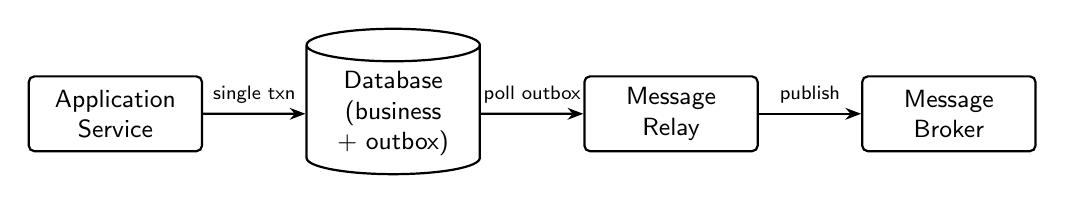
\begin{tikzpicture}[
    node distance=1.2cm,
    box/.style={draw, thick, minimum width=2.2cm, minimum height=0.95cm, align=center, rounded corners=2pt, font=\small},
    db/.style={draw, thick, cylinder, shape border rotate=90, aspect=0.25, minimum width=2.2cm, minimum height=1.4cm, align=center, font=\small},
    >={Stealth[length=2mm]}
]
\node[box] (app) {Application\\Service};
\node[db, right=1.3cm of app] (database) {Database\\(business\\+ outbox)};
\node[box, right=1.3cm of database] (relay) {Message\\Relay};
\node[box, right=1.3cm of relay] (broker) {Message\\Broker};

\draw[->, thick] (app)      -- node[above, font=\scriptsize] {single txn}  (database);
\draw[->, thick] (database) -- node[above, font=\scriptsize] {poll outbox} (relay);
\draw[->, thick] (relay)    -- node[above, font=\scriptsize] {publish}     (broker);
\end{tikzpicture}
\caption{Conceptual overview of the transactional outbox pattern.}
\label{fig:outbox-pattern}
\end{figure}

The platform developed in this project adopts the transactional outbox pattern in its webhook ingestion path. Each incoming webhook produces one \texttt{ZapRun} row and one \texttt{ZapRunOutbox} row, both inserted inside a single database transaction. A dedicated processor service, described in Chapter~4, is responsible for polling the outbox table and relaying its contents to Apache Kafka. The pattern provides the platform with \emph{at-least-once} delivery semantics for every webhook received, irrespective of transient failures in either the processor or the broker.

\section{Apache Kafka and Event Streaming}

Apache Kafka~\cite{kafka_docs} is a distributed, partitioned, replicated log that serves as the messaging backbone of the platform. Producers write records to named \emph{topics}, which are subdivided into \emph{partitions}; consumers belonging to a \emph{consumer group} read records from those partitions, with Kafka guaranteeing that each partition is consumed by at most one member of the group at any given time. Consumer offsets are stored inside Kafka itself, allowing a consumer to resume exactly where it left off after a restart.

Kafka was chosen over alternatives such as RabbitMQ or Redis Streams for three reasons that are directly relevant to this project. First, Kafka persists all records on disk for a configurable retention period, so messages survive consumer crashes and can be replayed during development and debugging. Second, Kafka's partitioning model provides a natural unit of horizontal scalability: adding more worker instances to the consumer group immediately distributes the load. Third, Kafka's wide industrial adoption means that the platform's operational patterns, such as consumer-group rebalancing, dead-letter queues and log compaction, map cleanly onto concepts already familiar to practitioners.

Figure~\ref{fig:kafka-pubsub} illustrates the basic publish-subscribe abstraction provided by Kafka. A \emph{producer} writes records into a named \emph{topic} (here, a topic called \emph{payment}), where each record is appended to the end of the log and assigned a monotonically increasing \emph{offset}. One or more \emph{consumers} read records from the topic at their own pace and track their progress using these offsets, which means that adding a new consumer never disturbs the existing ones. In the diagram, two independent consumers, ``Send SMS'' and ``Send Email'', each receive every record published to the topic.

\begin{figure}[h]
\centering
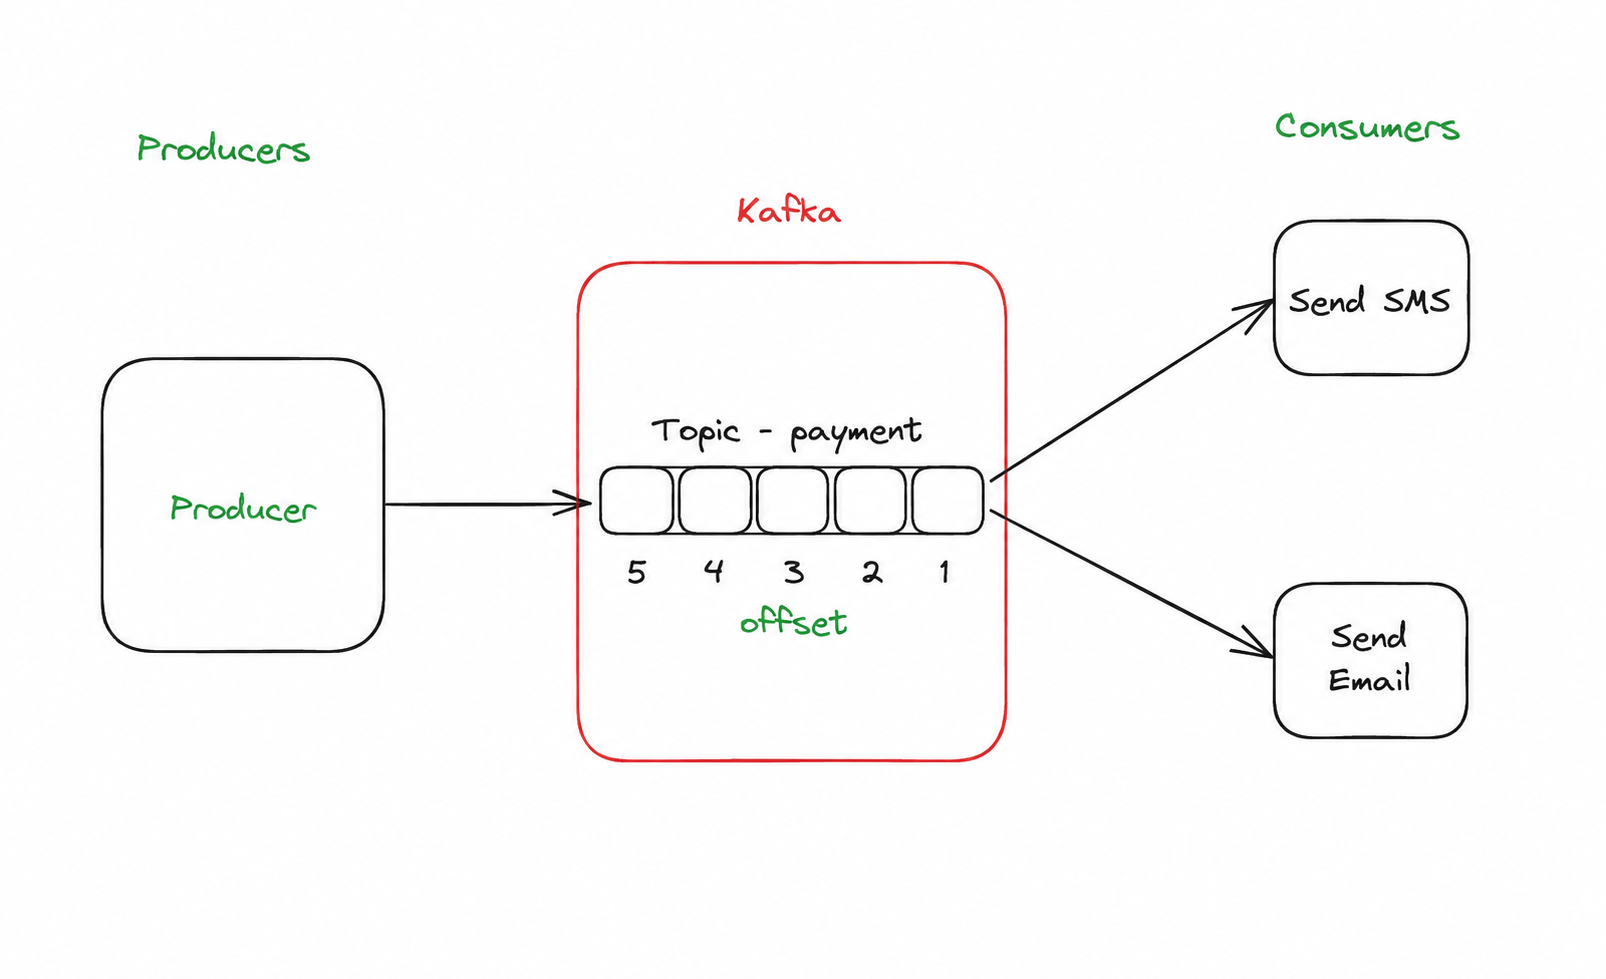
\includegraphics[width=0.85\textwidth]{figures/kafka-pub-sub.png}
\caption{Publish-subscribe model in Apache Kafka, with one producer, a single-partition topic and two independent consumers.}
\label{fig:kafka-pubsub}
\end{figure}

A practical example of how this abstraction enables decoupled, event-driven design is shown in Figure~\ref{fig:event-driven-flow}. A user-facing payment is recorded by a Node.js backend, which then writes a single event to Kafka. Three downstream services -- an email service, a mobile-SMS service and a push-notification service -- each independently consume that event and perform their respective side effects. The producer has no awareness of how many consumers exist or what they do, and additional consumers can be introduced later without modifying the producer. The platform developed in this project applies the same pattern: the processor service is the producer, and the worker service (which can be horizontally scaled) is the consumer of action events.

\begin{figure}[h]
\centering
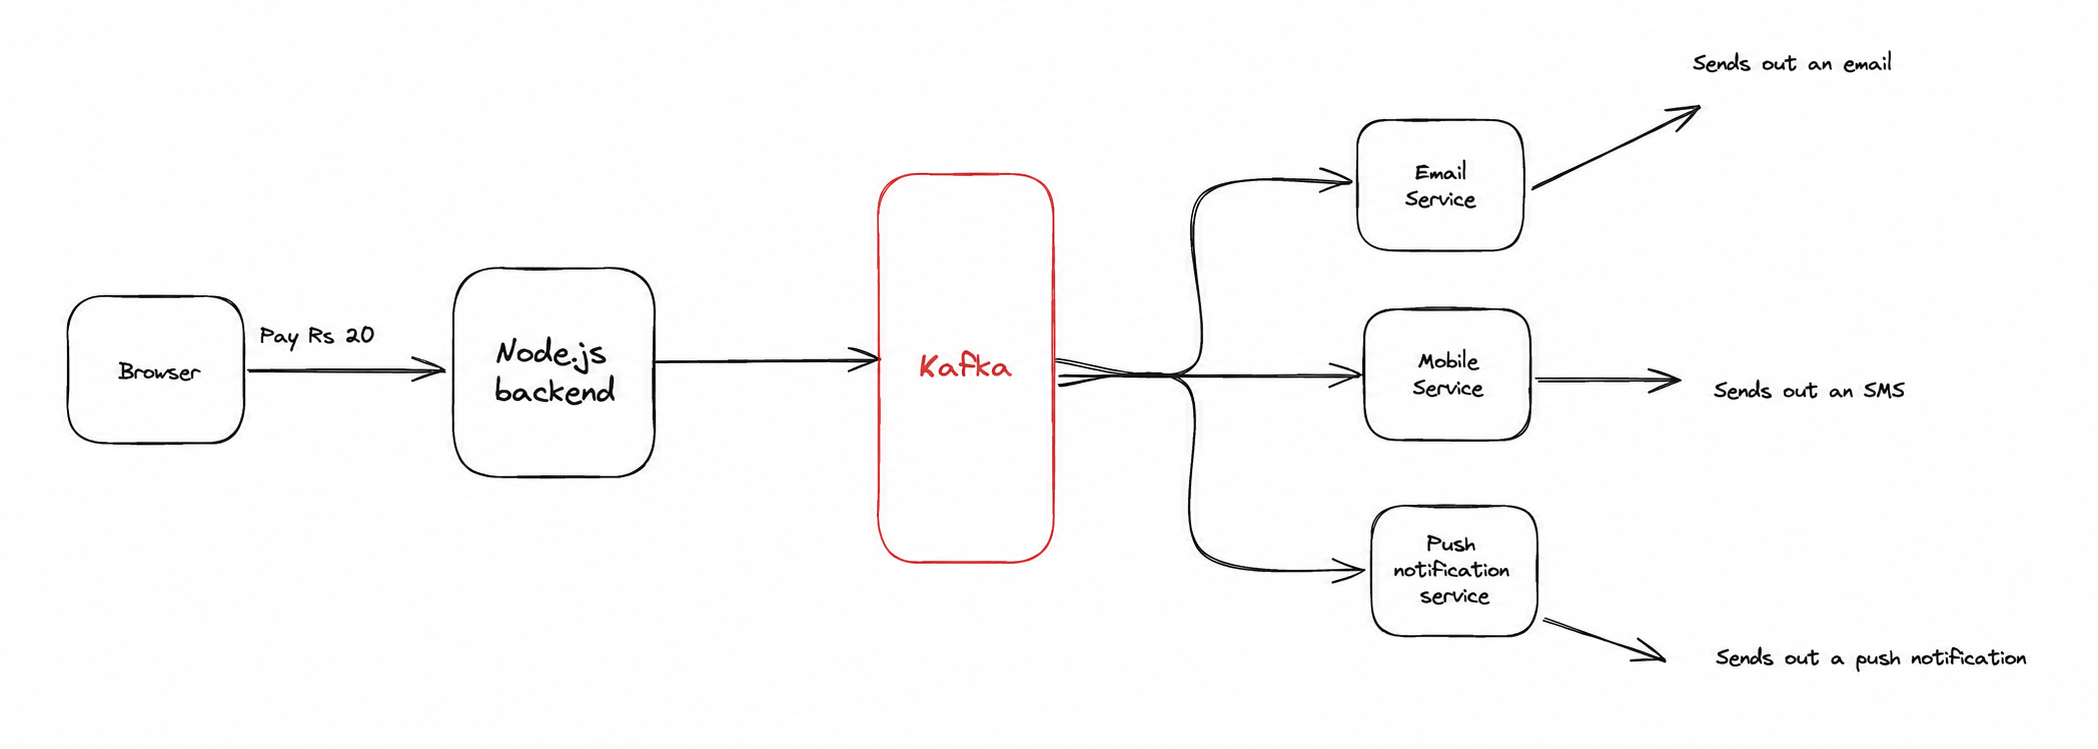
\includegraphics[width=\textwidth]{figures/event-driven-flow.png}
\caption{Event-driven fan-out via Kafka: a single payment event is consumed independently by an email service, a mobile service and a push-notification service.}
\label{fig:event-driven-flow}
\end{figure}

\section{Supporting Technologies}

The platform is built on top of several additional open-source technologies. The frontend is implemented using Next.js~\cite{nextjs_docs}, a React-based framework that supports both server-side rendering and static generation and provides built-in routing and API endpoints. The backend services are implemented in TypeScript on top of Node.js and the Express framework, with input validation performed using Zod schemas. Database access is mediated through Prisma ORM~\cite{prisma_docs}, which provides a fully typed query builder and an automatic migration system. Authentication is based on JSON Web Tokens~\cite{jones2015jwt}, with passwords hashed using the bcrypt algorithm. Transactional emails are sent using Nodemailer over standard SMTP, while blockchain actions interact with the Solana network through the \texttt{@solana/web3.js} library. The entire system is containerised using Docker and orchestrated locally with Docker Compose.
            % Chapter 2
\chapter{Problem Definition}

\section{Statement of the Problem}

The problem addressed in this project is the design and construction of a reliable, horizontally scalable workflow automation platform using open-source components, such that the platform can be self-hosted by an organisation, extended with new triggers and actions over time, and studied as a reference implementation of a modern event-driven microservices system.

Although workflow automation as a category is well established in the commercial market, the systems that dominate that market are proprietary and exhibit a number of limitations that motivate the alternative described here. First, they offer no control over the infrastructure on which the user's data is processed; sensitive payloads belonging to one organisation are routed through the shared infrastructure of a third party. Second, their pricing is based on the number of executed tasks, which renders very high-frequency automations economically unfeasible. Third, they cannot be customised at the source-code level, which prevents the integration of bespoke action types that interact with internal corporate systems. Finally, no commercial offering provides a transparent, fully open implementation that students of distributed systems can read, modify and run for instructional purposes.

The technical heart of the problem is therefore reliable event delivery: an arriving webhook event must be acknowledged quickly, must never be silently dropped, must be processed exactly once in the absence of failure (and at least once in the presence of failure), and must drive the sequential execution of an arbitrary chain of user-defined actions even though those actions may take significantly longer to complete than the original webhook request.

\section{Functional Requirements}

The platform must support the following functional requirements:

\begin{enumerate}[label=FR-\arabic*., leftmargin=*]
\item A user shall be able to register an account using an email address and a password.
\item A registered user shall be able to authenticate and receive a session token.
\item An authenticated user shall be able to create, list and view workflows (Zaps), each consisting of a trigger and one or more ordered actions.
\item Each created Zap shall be reachable through a unique public webhook URL that accepts an arbitrary JSON payload.
\item On receipt of a webhook, the platform shall record the event and shall execute the configured actions in the user-specified order.
\item The platform shall support at least two distinct action types: sending a transactional email and sending a Solana cryptocurrency transfer.
\item Action metadata shall support template substitution from the webhook payload so that user-supplied strings such as ``\texttt{Hello \{user.name\}}'' resolve at execution time.
\item The list of available trigger and action types shall be exposed to the frontend so that the Zap-builder UI is data-driven.
\end{enumerate}

\section{Non-Functional Requirements}

In addition, the platform shall satisfy the following non-functional requirements:

\begin{enumerate}[label=NFR-\arabic*., leftmargin=*]
\item \textbf{Durability.} No webhook event that has been acknowledged with an HTTP 200 response may be lost, even if downstream components (the message broker, the worker) are temporarily unavailable at the time the webhook is received.
\item \textbf{At-least-once execution.} Each configured action of an accepted Zap run must eventually execute, even if the worker crashes mid-execution. Duplicate execution of an action under failure conditions is acceptable.
\item \textbf{Ordered execution.} The actions of a single Zap run must execute in the order specified by the \texttt{sortingOrder} of the action records.
\item \textbf{Horizontal scalability.} The webhook-receiving service, the API service and the worker service must each be independently replicable so that additional capacity can be added without architectural change.
\item \textbf{Statelessness of service replicas.} Replicas of the API, hook and worker services must share no in-memory state other than the contents of the database and the Kafka log.
\item \textbf{Operability.} The full system must run with a single \texttt{docker compose up} on a developer machine, and must be deployable to a single production virtual machine without manual coordination between services.
\item \textbf{Security.} Passwords must be stored only in salted, hashed form. Authenticated endpoints must reject requests that do not present a valid token. Action secrets (SMTP credentials, blockchain private key) must be configurable through environment variables rather than committed to source.
\end{enumerate}

\section{Constraints and Assumptions}

The implementation operates under the following constraints and assumptions:

\begin{itemize}
\item Only a single trigger type, namely an incoming HTTP webhook, is implemented in this iteration. Polling triggers and scheduled triggers are deferred to future work.
\item Only two action types, email and Solana transfer, are implemented. The architecture, however, does not preclude additional action types from being added without schema change because all action-specific parameters are stored in a JSON metadata column.
\item The deployment target is a single virtual machine running Docker Compose; a Kubernetes deployment is out of scope. The architecture assumes a single PostgreSQL instance and a single Kafka broker, both of which are sufficient for the expected workload of this iteration.
\item Webhook payloads are assumed to be JSON and to fit within the body-size limits imposed by the Express framework's default body parser.
\item External services (the SMTP provider and the Solana RPC endpoint) are assumed to be available; transient unavailability is handled by Kafka redelivery, but persistent unavailability is reported as a worker error and left for human investigation.
\end{itemize}

\section{Significance of the Problem}

Solving this problem produces three concrete outcomes. The first is a usable workflow automation tool that an individual or a small organisation can deploy in-house, free of recurring per-task licence costs, with full control over the data being processed. The second is an open codebase that demonstrates the practical application of the transactional outbox pattern, event streaming, and stateless microservice replication, all in a domain whose business logic is intuitive enough to make the architectural choices clearly visible. The third, more general outcome is a body of design and implementation experience for the project team, covering distributed systems, asynchronous programming, relational schema design, container orchestration and continuous deployment, all of which are directly applicable to professional software engineering practice.
    % Chapter 3
\chapter{Proposed Solution}

\section{System Overview}

The platform is implemented as a set of five independently deployable services that communicate either over HTTP or through an Apache Kafka topic. The five services are the \emph{frontend}, the \emph{primary backend}, the \emph{hook} service, the \emph{processor} service and the \emph{worker} service. A shared PostgreSQL database serves as the system of record for all persistent state, and Kafka is used as the asynchronous channel that carries action events between the processor and the worker. A high-level view of the system is shown in Figure~\ref{fig:architecture}.

\begin{figure}[h]
\centering
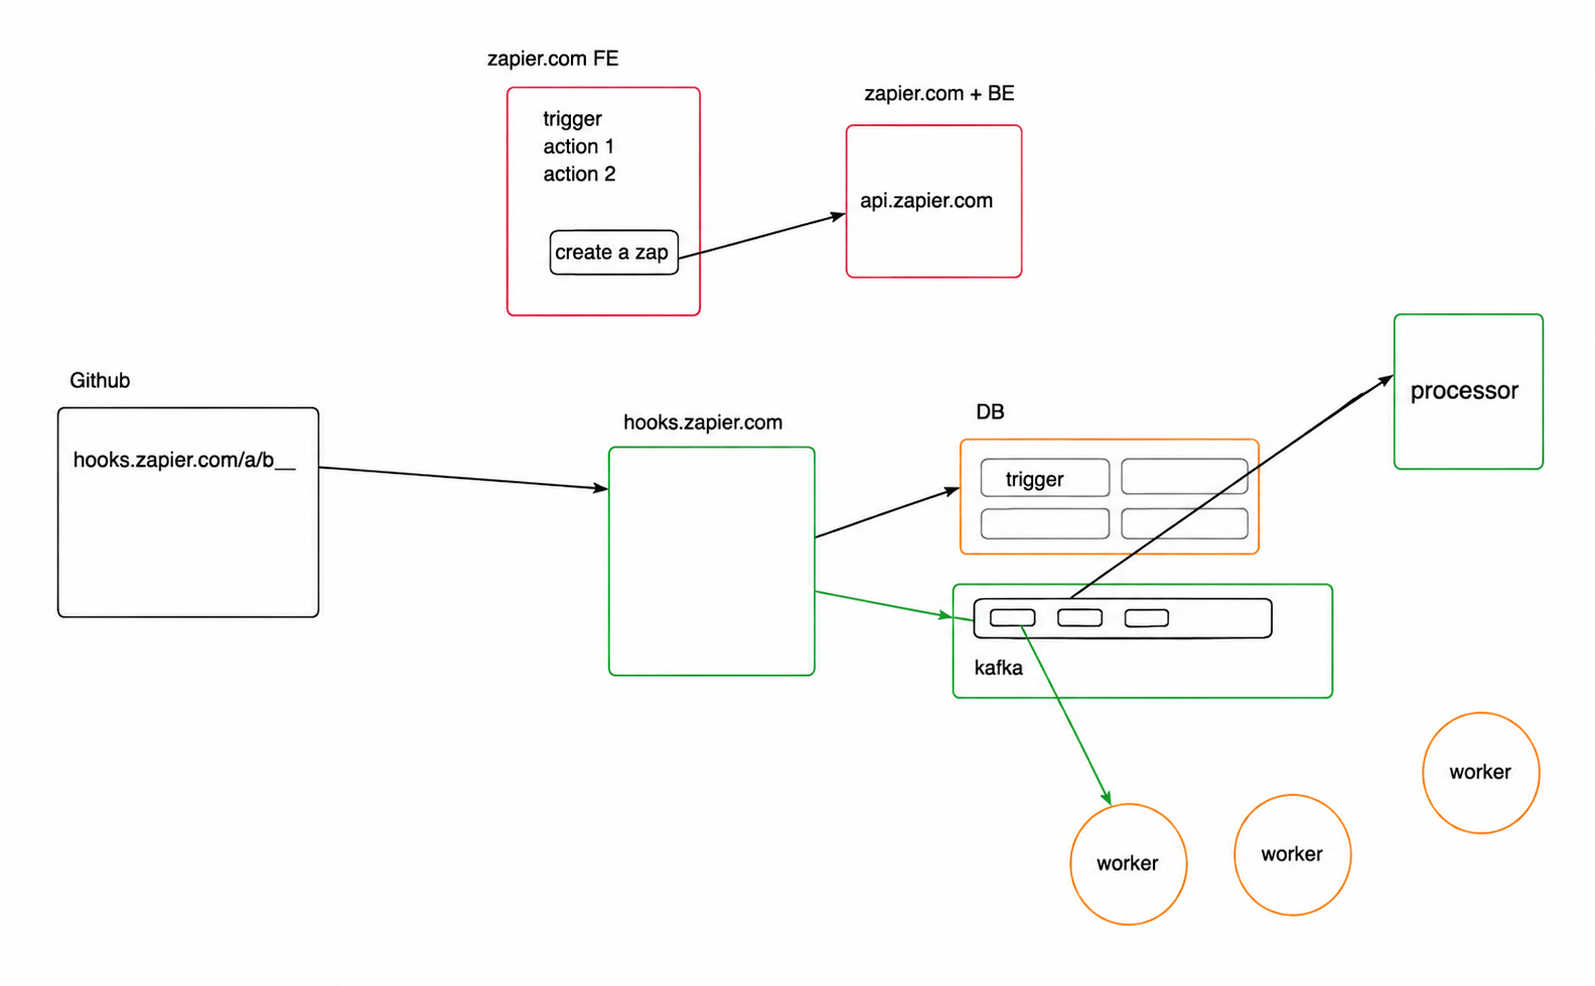
\includegraphics[width=0.95\textwidth]{figures/system-architecture.png}
\caption{High-level architecture of the platform.}
\label{fig:architecture}
\end{figure}

The diagram is organised around two complementary flows. The upper portion shows the \emph{authoring} flow: the user composes a trigger and one or more actions in the frontend (\texttt{zapier.com FE}) and submits the assembled workflow to the primary backend (\texttt{api.zapier.com}), which persists it to the database. The lower portion shows the \emph{execution} flow: an external system (illustrated in the diagram as a GitHub webhook posting to \texttt{hooks.zapier.com/a/b\_\_}) invokes the public URL served by the hook service, which records the event in the database; the processor then relays each new event from the database into Kafka; and a horizontally scalable pool of worker consumers reads from Kafka and executes the configured actions. For visual clarity the diagram omits the read-only database accesses performed by the primary backend when serving API requests and by the worker when loading the Zap definition before each action; both are described in the corresponding service sections later in this chapter.

The end-to-end lifecycle of a single workflow execution proceeds as follows. A user first authenticates against the primary backend through the frontend, creates a workflow, and receives a unique public webhook URL bound to that workflow. When that URL is later invoked by an external system, the hook service accepts the request and persists a \texttt{ZapRun} row together with a \texttt{ZapRunOutbox} row in a single database transaction. The processor service continuously polls the outbox table and, for each entry it finds, produces a corresponding message to the \texttt{zap-events} Kafka topic before deleting the outbox row. The worker service consumes messages from that topic; for each message it loads the relevant workflow definition, executes the appropriate action (e.g.\ email or Solana transfer), and if the workflow has further actions remaining, republishes the same message with an incremented stage number so that the next action can be processed by the same consumer group. Figure~\ref{fig:webhook-sequence} traces the corresponding sequence of messages between the services for a single Zap run.

\begin{figure}[h]
\centering
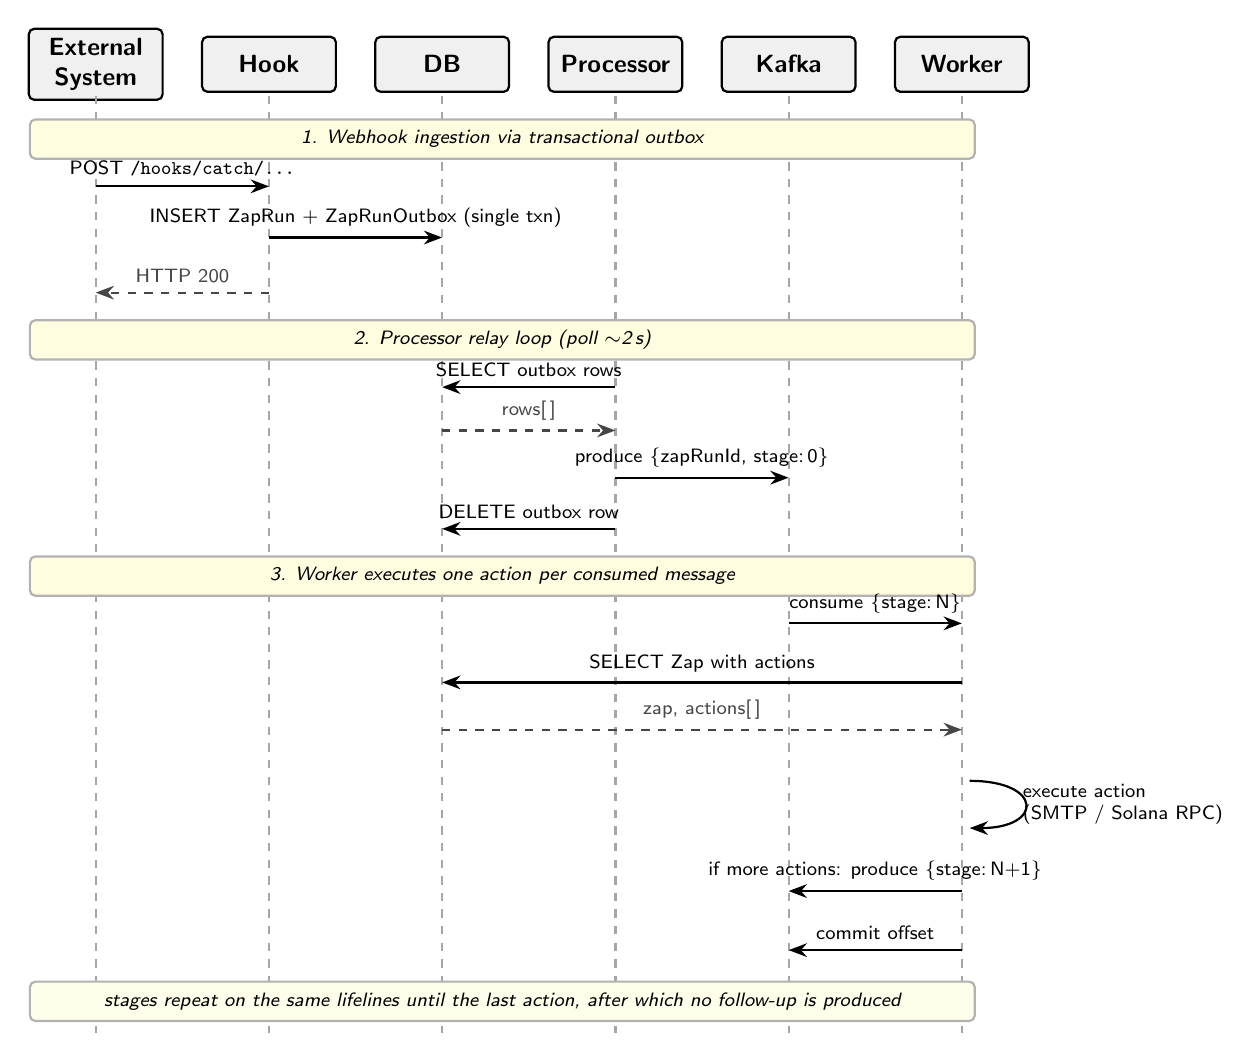
\begin{tikzpicture}[
    actor/.style={draw, thick, rounded corners=2pt, minimum width=1.7cm, minimum height=0.7cm, align=center, font=\small\bfseries, fill=gray!12},
    lifeline/.style={dashed, gray!70, thick},
    msg/.style={->, thick, >=Stealth, font=\scriptsize},
    msgret/.style={->, thick, dashed, >=Stealth, gray!55!black, font=\scriptsize},
    phase/.style={draw=gray!60, thick, rounded corners=2pt, minimum height=0.5cm, font=\scriptsize\itshape, align=left, fill=yellow!12, inner sep=3pt}
]
\def\xExt{0}
\def\xHook{2.2}
\def\xDb{4.4}
\def\xProc{6.6}
\def\xKafka{8.8}
\def\xWorker{11.0}

% Actor headers
\node[actor] (ext)    at (\xExt,    0) {External\\System};
\node[actor] (hook)   at (\xHook,   0) {Hook};
\node[actor] (db)     at (\xDb,     0) {DB};
\node[actor] (proc)   at (\xProc,   0) {Processor};
\node[actor] (kafka)  at (\xKafka,  0) {Kafka};
\node[actor] (worker) at (\xWorker, 0) {Worker};

% Lifelines
\foreach \x in {\xExt, \xHook, \xDb, \xProc, \xKafka, \xWorker} {
    \draw[lifeline] (\x, -0.4) -- (\x, -12.3);
}

% --- Phase 1: Webhook ingestion ---
\node[phase, anchor=west, minimum width=12cm] at (-0.85, -0.95) {1. Webhook ingestion via transactional outbox};

\draw[msg]    (\xExt,  -1.55) -- node[above] {POST \texttt{/hooks/catch/...}} (\xHook, -1.55);
\draw[msg]    (\xHook, -2.20) -- node[above] {INSERT ZapRun + ZapRunOutbox (single txn)} (\xDb, -2.20);
\draw[msgret] (\xHook, -2.90) -- node[above] {HTTP 200} (\xExt, -2.90);

% --- Phase 2: Processor relay ---
\node[phase, anchor=west, minimum width=12cm] at (-0.85, -3.50) {2. Processor relay loop (poll $\sim$2\,s)};

\draw[msg]    (\xProc, -4.10) -- node[above] {SELECT outbox rows} (\xDb, -4.10);
\draw[msgret] (\xDb,   -4.65) -- node[above] {rows[\,]} (\xProc, -4.65);
\draw[msg]    (\xProc, -5.25) -- node[above] {produce \{zapRunId, stage:\,0\}} (\xKafka, -5.25);
\draw[msg]    (\xProc, -5.90) -- node[above] {DELETE outbox row} (\xDb, -5.90);

% --- Phase 3: Worker execution ---
\node[phase, anchor=west, minimum width=12cm] at (-0.85, -6.50) {3. Worker executes one action per consumed message};

\draw[msg]    (\xKafka,  -7.10) -- node[above] {consume \{stage:\,N\}} (\xWorker, -7.10);
\draw[msg]    (\xWorker, -7.85) -- node[above] {SELECT Zap with actions} (\xDb, -7.85);
\draw[msgret] (\xDb,     -8.45) -- node[above] {zap, actions[\,]} (\xWorker, -8.45);

% Self-message on Worker: outbound call to external action service
\draw[msg, ->, thick] (\xWorker + 0.1, -9.10) to[out=0, in=0, looseness=4] (\xWorker + 0.1, -9.70);
\node[font=\scriptsize, anchor=west, align=left] at (\xWorker + 0.65, -9.40) {execute action\\(SMTP / Solana RPC)};

\draw[msg] (\xWorker, -10.50) -- node[above] {if more actions: produce \{stage:\,N+1\}} (\xKafka, -10.50);
\draw[msg] (\xWorker, -11.25) -- node[above] {commit offset} (\xKafka, -11.25);

% Closing note
\node[phase, anchor=west, minimum width=12cm, fill=yellow!8] at (-0.85, -11.90) {stages repeat on the same lifelines until the last action, after which no follow-up is produced};

\end{tikzpicture}
\caption{End-to-end sequence of messages for a single Zap run, from external webhook reception through action execution. Solid arrows denote synchronous calls; dashed arrows denote return values. The self-arrow on the \emph{Worker} lifeline represents the outbound call to the external service that the chosen action targets (SMTP relay for the \texttt{email} action or Solana RPC for the \texttt{send-sol} action).}
\label{fig:webhook-sequence}
\end{figure}

This division of responsibilities directly addresses the functional and non-functional requirements stated in Chapter~3. Durability of accepted events is provided by the transactional outbox table; ordered, at-least-once execution of actions is provided by the combination of the \texttt{sortingOrder} field and Kafka's manual offset commits; horizontal scalability of the worker is provided by Kafka's consumer-group abstraction; and the operability requirement is met by packaging every service as a Docker container that is brought up from a single Compose file.

\section{Database Design}

All persistent state is stored in a single PostgreSQL database whose schema is managed by Prisma migrations. The schema comprises seven tables, summarised in Table~\ref{tab:schema}.

\begin{table}[h]
\centering
\caption{Core tables of the database schema.}
\label{tab:schema}
\renewcommand{\arraystretch}{1.3}
\begin{tabular}{|p{3.2cm}|p{10cm}|}
\hline
\textbf{Table} & \textbf{Purpose} \\ \hline
\texttt{User} & Stores registered users. Fields: \texttt{id}, \texttt{name}, \texttt{email}, \texttt{password} (bcrypt-hashed). \\ \hline
\texttt{Zap} & Represents a single workflow owned by a user. Holds references to the associated trigger and actions. \\ \hline
\texttt{AvailableTrigger} & Catalogue of trigger types known to the platform (currently only ``webhook''). \\ \hline
\texttt{Trigger} & Concrete trigger instance attached to a single Zap, with a JSON \texttt{metadata} column for configuration. \\ \hline
\texttt{AvailableAction} & Catalogue of action types known to the platform (email, send-sol). \\ \hline
\texttt{Action} & Concrete action instance attached to a Zap, with \texttt{metadata} and a \texttt{sortingOrder} that defines execution position. \\ \hline
\texttt{ZapRun} & One row per execution of a Zap, carrying the webhook payload in a JSON \texttt{metadata} column. \\ \hline
\texttt{ZapRunOutbox} & Transactional outbox row associated with a single \texttt{ZapRun}. Inserted in the same transaction as the \texttt{ZapRun} and later deleted by the processor. \\ \hline
\end{tabular}
\end{table}

The use of a JSON column for trigger and action metadata is a deliberate design choice: it allows new trigger and action types to be added to the catalogue without any schema migration, since each type is free to define the shape of its own metadata. Only the skeleton of the relational model, with its foreign-key constraints, is enforced at the database level. The separation between \texttt{AvailableAction} (the type) and \texttt{Action} (the instance) is analogous to the separation between a class and its instances in an object-oriented language. The full entity-relationship diagram for the schema, generated from the live Prisma model, is shown in Figure~\ref{fig:schema-er}.

\begin{figure}[h]
\centering
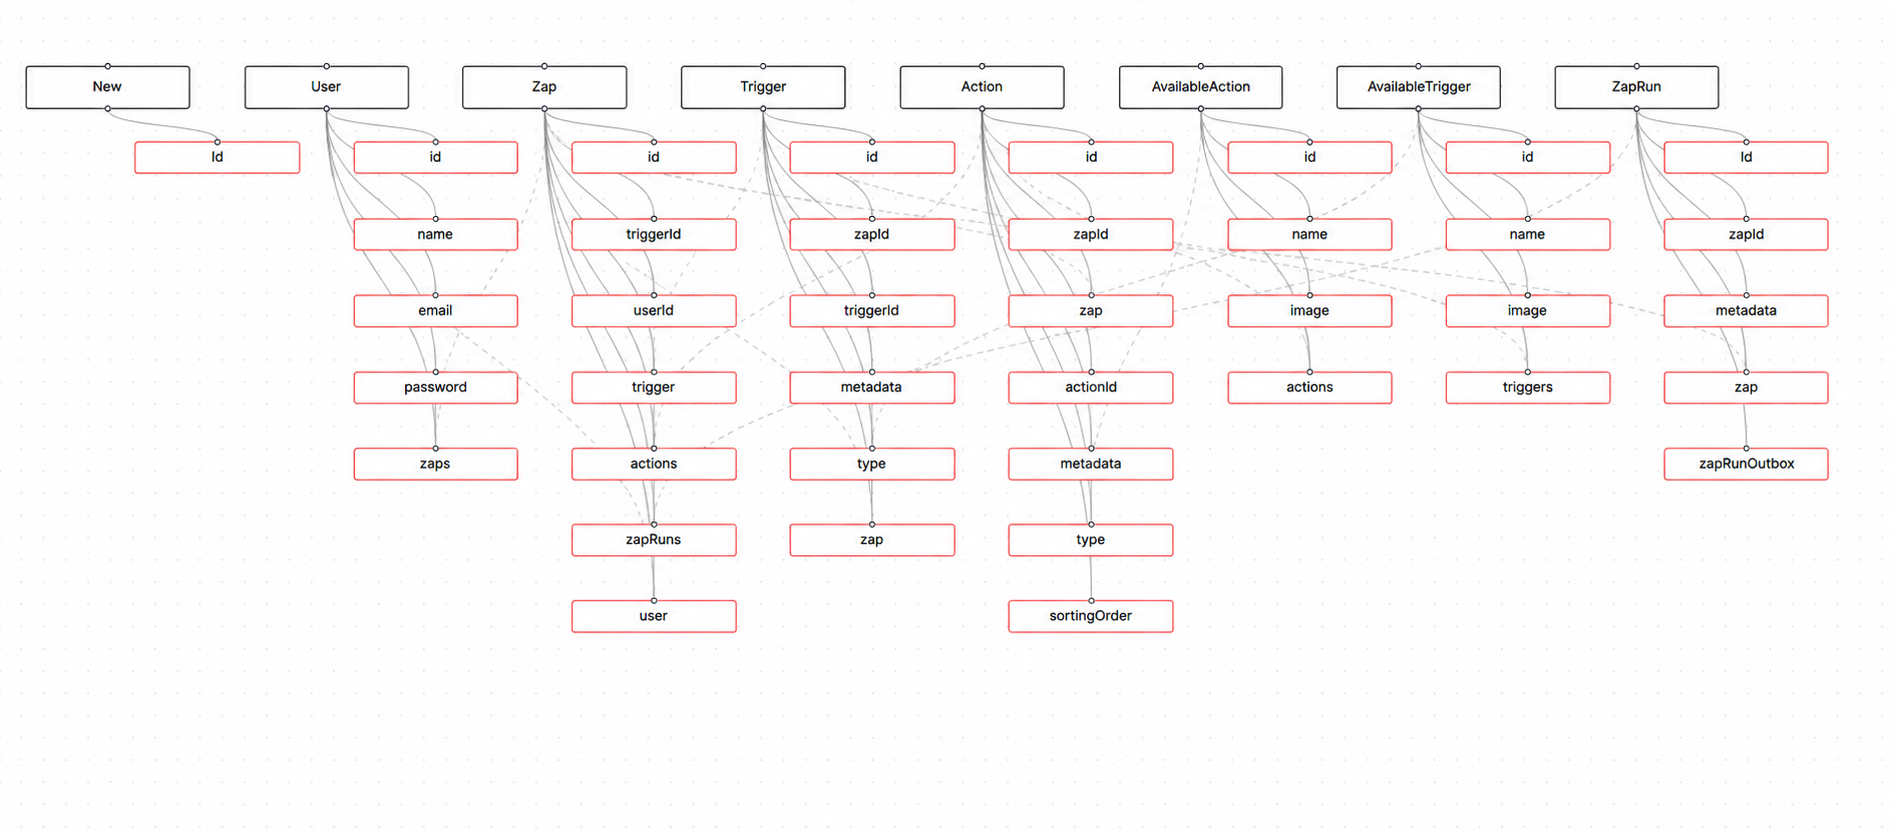
\includegraphics[width=\textwidth]{figures/database-schema.png}
\caption{Entity-relationship diagram of the database schema.}
\label{fig:schema-er}
\end{figure}

\section{Primary Backend Service}

The primary backend is an Express application written in TypeScript. It is the only service that frontend clients communicate with, and it is responsible for authentication and for all create / read operations on user-owned resources. All input is validated against Zod schemas before any business logic executes, and the resulting typed objects are passed to Prisma for persistence. Authentication is handled by a middleware function that extracts a JSON Web Token from the \texttt{Authorization} header, verifies it against a secret, and attaches the decoded user identifier to the request object for downstream handlers. Figure~\ref{fig:login-network} shows the browser developer-tools view of a sign-in request being issued against the local backend, with the underlying \texttt{POST /api/v1/user/signin} call visible in the Network panel. The REST endpoints exposed by the service are summarised in Table~\ref{tab:endpoints}.

\begin{figure}[h]
\centering
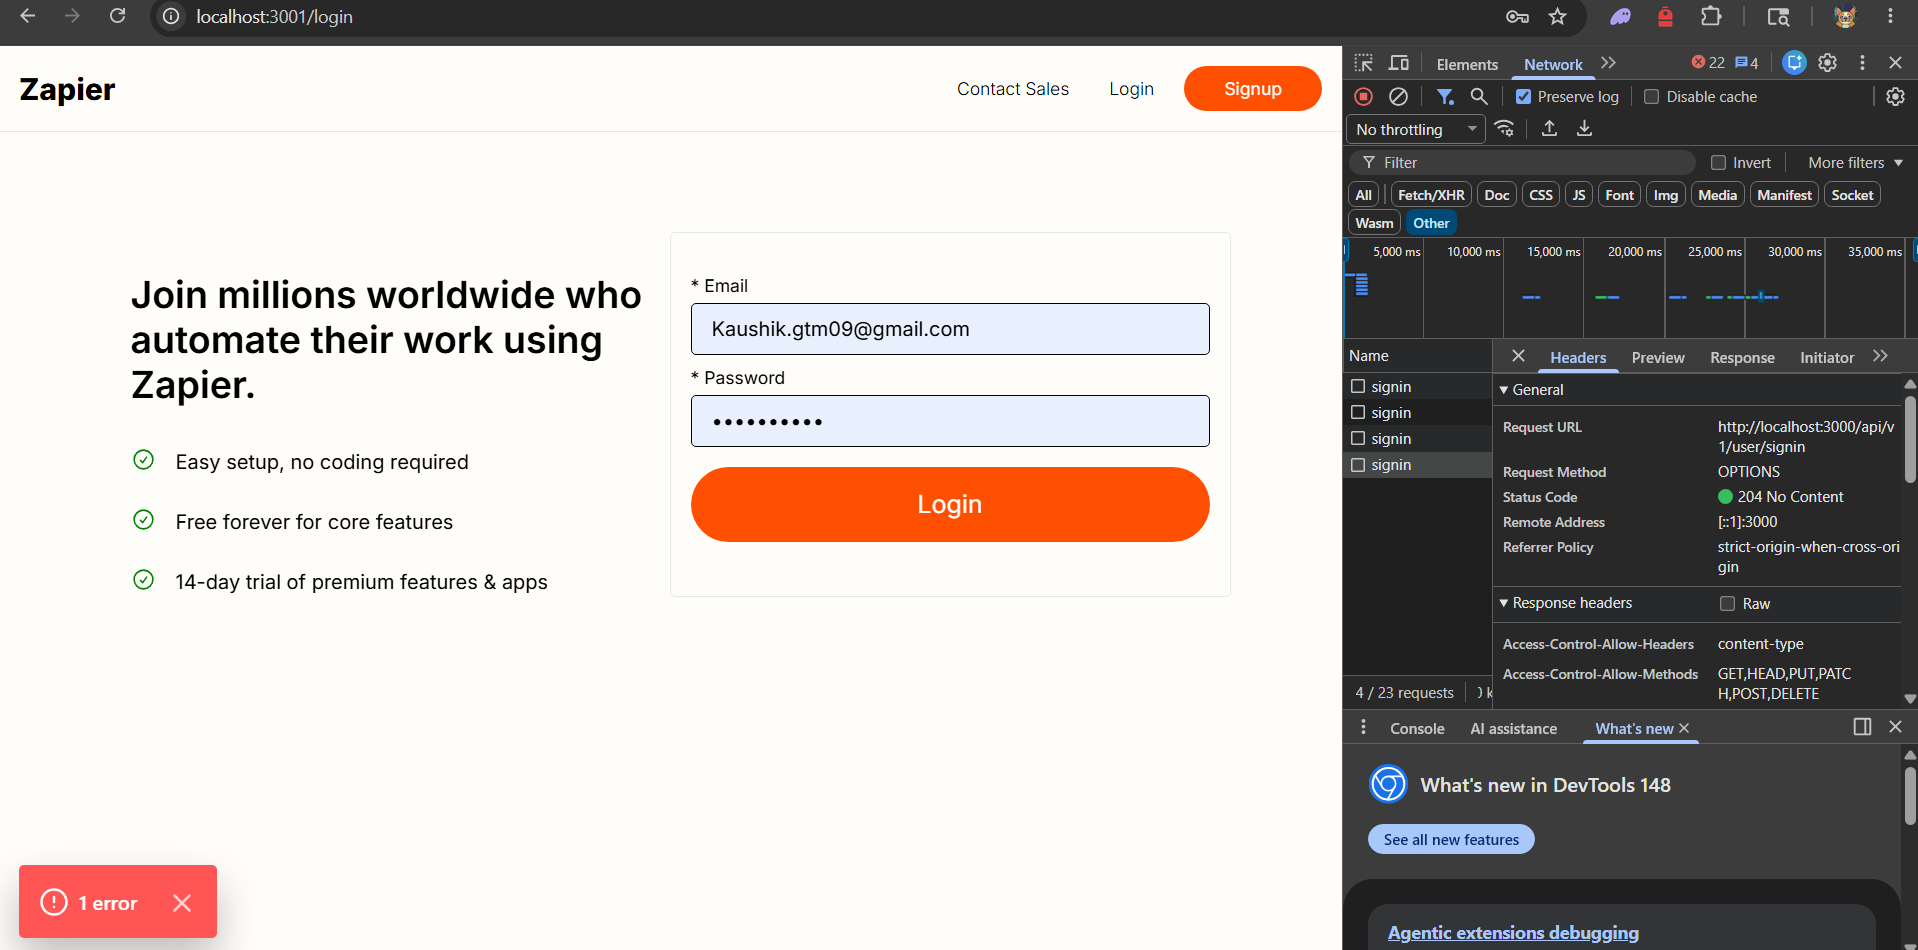
\includegraphics[width=0.95\textwidth]{figures/ui-login-network.png}
\caption{Sign-in request as observed in the browser developer tools. The login form on the left invokes \texttt{POST /api/v1/user/signin} against the primary backend; the request and response are visible in the Network panel on the right, demonstrating that the authentication endpoint is reachable and returning a token.}
\label{fig:login-network}
\end{figure}

\begin{table}[h]
\centering
\caption{REST endpoints exposed by the primary backend.}
\label{tab:endpoints}
\renewcommand{\arraystretch}{1.3}
\begin{tabular}{|l|p{4.2cm}|c|p{5.0cm}|}
\hline
\textbf{Method} & \textbf{Path} & \textbf{Auth} & \textbf{Purpose} \\ \hline
POST & \texttt{/api/v1/user/signup} & No & Register a new user. \\ \hline
POST & \texttt{/api/v1/user/signin} & No & Authenticate and issue a JWT. \\ \hline
GET & \texttt{/api/v1/user} & Yes & Fetch the authenticated user's profile. \\ \hline
POST & \texttt{/api/v1/zap} & Yes & Create a new Zap with trigger and actions. \\ \hline
GET & \texttt{/api/v1/zap} & Yes & List all Zaps owned by the user. \\ \hline
GET & \texttt{/api/v1/zap/:zapId} & Yes & Fetch a single Zap including its actions. \\ \hline
GET & \texttt{/api/v1/trigger/available} & No & List all available trigger types. \\ \hline
GET & \texttt{/api/v1/action/available} & No & List all available action types. \\ \hline
\end{tabular}
\end{table}

The \texttt{POST /api/v1/zap} handler is worth describing in detail because it coordinates multiple table inserts. It begins a single Prisma transaction in which it first creates the \texttt{Zap} row with an empty \texttt{triggerId}, then creates all of the requested \texttt{Action} rows with appropriate \texttt{sortingOrder} values, then creates the \texttt{Trigger} row that references the \texttt{Zap}, and finally updates the \texttt{Zap.triggerId} field to point at the newly created trigger. Because all four operations are executed inside a single transaction, the database is never observed in a partially constructed state.

\section{Hook Service}

The hook service is a minimal Express application whose sole responsibility is to receive webhook requests from external systems and enqueue them for asynchronous processing. It exposes a single endpoint, \texttt{POST /hooks/catch/:userId/:zapId}, which accepts an arbitrary JSON body and returns a short acknowledgement. For every request received, it executes a single Prisma transaction that inserts one row into \texttt{ZapRun} (carrying the incoming payload in the \texttt{metadata} column) and one row into \texttt{ZapRunOutbox} (referencing the \texttt{ZapRun}). A simplified version of the relevant code is shown in Listing~\ref{lst:hook}.

\begin{lstlisting}[language=JavaScript, caption={Transactional outbox insert in the hook service.}, label=lst:hook]
app.post("/hooks/catch/:userId/:zapId", async (req, res) => {
    const { userId, zapId } = req.params;
    const body = req.body;
    await client.$transaction(async (tx) => {
        const run = await tx.zapRun.create({
            data: { zapId, metadata: body }
        });
        await tx.zapRunOutbox.create({
            data: { zapRunId: run.id }
        });
    });
    res.json({ message: "webhook received" });
});
\end{lstlisting}

The design consequence of this pattern is that, from the moment the transaction commits, the platform has accepted responsibility for eventually executing the associated actions. Neither the processor nor the Kafka cluster needs to be reachable at the instant the webhook arrives. Should the processor be down, the \texttt{ZapRunOutbox} rows simply accumulate in the database; when the processor resumes, it drains the backlog and the platform catches up.

\section{Processor Service}

The processor is a headless Node.js service that continuously polls the \texttt{ZapRunOutbox} table, relays the contents to Kafka and deletes the processed rows. Its control loop is intentionally simple: on each iteration it fetches up to ten outbox rows; if none are found, it sleeps for two seconds and tries again; if rows are found, it produces a message for each row to the \texttt{zap-events} Kafka topic and then performs a \texttt{deleteMany} on the rows it just sent. Messages have the JSON shape \texttt{\{"zapRunId": <uuid>, "stage": 0\}}, where the \texttt{stage} field indicates which position in the action chain should be executed next.

Because the polling query and the delete are not wrapped in a transaction with the producer's \texttt{send} call, in principle a crash between the send and the delete could cause an outbox row to be published twice. The platform accepts this \emph{at-least-once} delivery semantic deliberately: the worker is idempotent in practice because it identifies its work by \texttt{zapRunId} and \texttt{stage}, and duplicate executions of an action (e.g.\ sending the same email twice) are considered acceptable given the target use-case. An at-most-once alternative would require a two-phase commit that is not justified by the present requirements.

\section{Worker Service}

The worker is a Kafka consumer that performs the actual execution of actions. It joins the consumer group \texttt{main-worker-2} and subscribes to the \texttt{zap-events} topic. Automatic offset commits are disabled; the worker only commits offsets after the action has been successfully executed, so that in the event of a crash the failed message is re-delivered on restart. The worker currently supports two action types, described in Table~\ref{tab:actions}.

\begin{table}[h]
\centering
\caption{Action types supported by the worker.}
\label{tab:actions}
\renewcommand{\arraystretch}{1.3}
\begin{tabular}{|l|p{4.5cm}|p{7cm}|}
\hline
\textbf{Action ID} & \textbf{Metadata fields} & \textbf{Behaviour} \\ \hline
\texttt{email} & \texttt{email}, \texttt{body} & Sends a transactional email over SMTP using Nodemailer to the recipient address after placeholder substitution against the webhook payload. \\ \hline
\texttt{send-sol} & \texttt{address}, \texttt{amount} & Constructs and signs a Solana transfer transaction using the \texttt{@solana/web3.js} library, then submits it to the Solana mainnet RPC endpoint. \\ \hline
\end{tabular}
\end{table}

For every consumed message the worker loads the corresponding \texttt{Zap} together with its actions from the database, selects the action whose \texttt{sortingOrder} equals the message's \texttt{stage}, and executes it. Before execution, the action's metadata (which may contain placeholders such as \texttt{\{payment.amount\}}) is passed through a simple template parser that substitutes values taken from the webhook payload stored on the \texttt{ZapRun}. If the current stage is not the last action of the Zap, the worker produces a follow-up message to the same Kafka topic with an incremented stage, thereby driving the next step of the workflow. If the current stage is the last, no follow-up is produced and the offset is committed. Figure~\ref{fig:worker-stages} illustrates this self-republishing loop for a three-action Zap.

\begin{figure}[h]
\centering
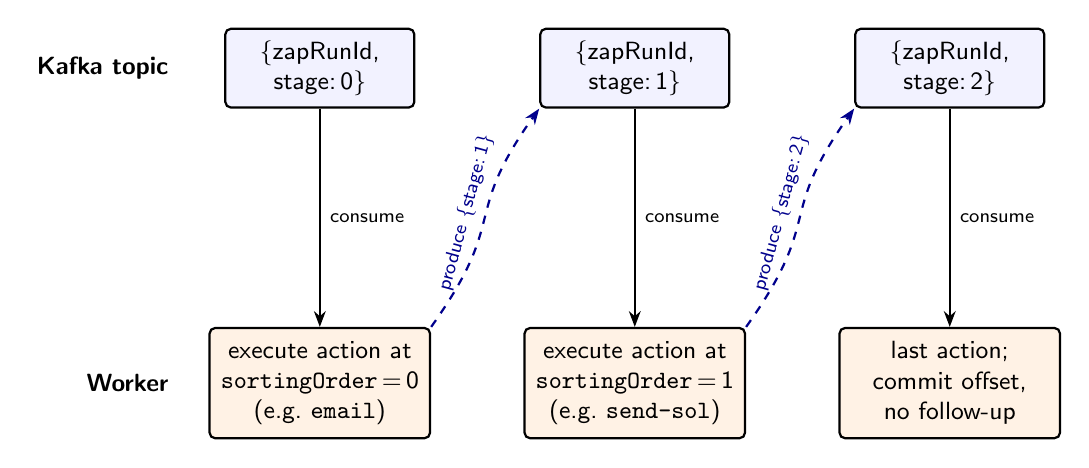
\begin{tikzpicture}[
    msg/.style={draw, thick, rounded corners=2pt, minimum width=2.4cm, minimum height=1.0cm, align=center, font=\small, fill=blue!5},
    worker/.style={draw, thick, rounded corners=2pt, minimum width=2.8cm, minimum height=1.4cm, align=center, font=\small, fill=orange!10},
    lanelabel/.style={font=\bfseries\small, align=right, anchor=east},
    >={Stealth[length=2mm]}
]
% Lane labels
\node[lanelabel] at (-1.8, 2.1) {Kafka topic};
\node[lanelabel] at (-1.8, -1.9) {Worker};

% Messages on the topic
\node[msg] (m0) at (0, 2.1) {\{zapRunId,\\ stage:\,0\}};
\node[msg] (m1) at (4, 2.1) {\{zapRunId,\\ stage:\,1\}};
\node[msg] (m2) at (8, 2.1) {\{zapRunId,\\ stage:\,2\}};

% Worker iterations
\node[worker] (w0) at (0, -1.9) {execute action at\\ \texttt{sortingOrder}\,=\,0\\ (e.g.\ \texttt{email})};
\node[worker] (w1) at (4, -1.9) {execute action at\\ \texttt{sortingOrder}\,=\,1\\ (e.g.\ \texttt{send-sol})};
\node[worker] (w2) at (8, -1.9) {last action;\\ commit offset,\\ no follow-up};

% Consume arrows (Kafka -> Worker)
\draw[->, thick] (m0) -- node[right, font=\scriptsize] {consume} (w0);
\draw[->, thick] (m1) -- node[right, font=\scriptsize] {consume} (w1);
\draw[->, thick] (m2) -- node[right, font=\scriptsize] {consume} (w2);

% Produce arrows (Worker -> Kafka, with stage+1)
\draw[->, thick, blue!55!black, dashed]
  (w0.north east) .. controls +(1.0,1.4) and +(-1.0,-1.4) ..
  node[midway, sloped, above, font=\scriptsize] {produce \{stage:\,1\}} (m1.south west);
\draw[->, thick, blue!55!black, dashed]
  (w1.north east) .. controls +(1.0,1.4) and +(-1.0,-1.4) ..
  node[midway, sloped, above, font=\scriptsize] {produce \{stage:\,2\}} (m2.south west);
\end{tikzpicture}
\caption{Sequential execution of a three-action Zap through worker self-republishing. Each consumed message at \texttt{stage}\,$=N$ causes the worker to execute the action whose \texttt{sortingOrder}\,$=N$; if further actions remain the worker produces a follow-up message with \texttt{stage}\,$=N{+}1$ to the same Kafka topic. On the final action no follow-up is produced and the consumer-group offset is committed.}
\label{fig:worker-stages}
\end{figure}

This design keeps the worker entirely stateless between messages. All progress is tracked by the combination of the Kafka offset and the \texttt{stage} field inside the message. A worker crash therefore cannot cause an action to be skipped: either the offset was committed (and the action was executed) or it was not (and the message will be re-delivered).

\section{Frontend and Deployment}

The frontend is a Next.js application written in TypeScript and styled with Tailwind CSS. It consists of four principal pages: a landing page, a sign-up form, a sign-in form, and a dashboard, illustrated in Figures~\ref{fig:ui-public} and~\ref{fig:ui-auth}. From the dashboard the user can list existing Zaps, copy their unique public webhook URL, and navigate to a Zap-builder screen. The Zap builder, shown in Figure~\ref{fig:ui-zap-builder}, fetches the catalogues of available triggers and actions from the primary backend, and lets the user assemble a workflow visually by clicking a trigger and then appending actions one at a time. Each action presents a small form whose fields are determined by the action type; the form values become the JSON \texttt{metadata} stored on the \texttt{Action} row. Submitting the builder issues a single \texttt{POST /api/v1/zap} call to the backend.

\begin{figure}[h]
\centering
\begin{minipage}[t]{0.48\textwidth}
    \centering
    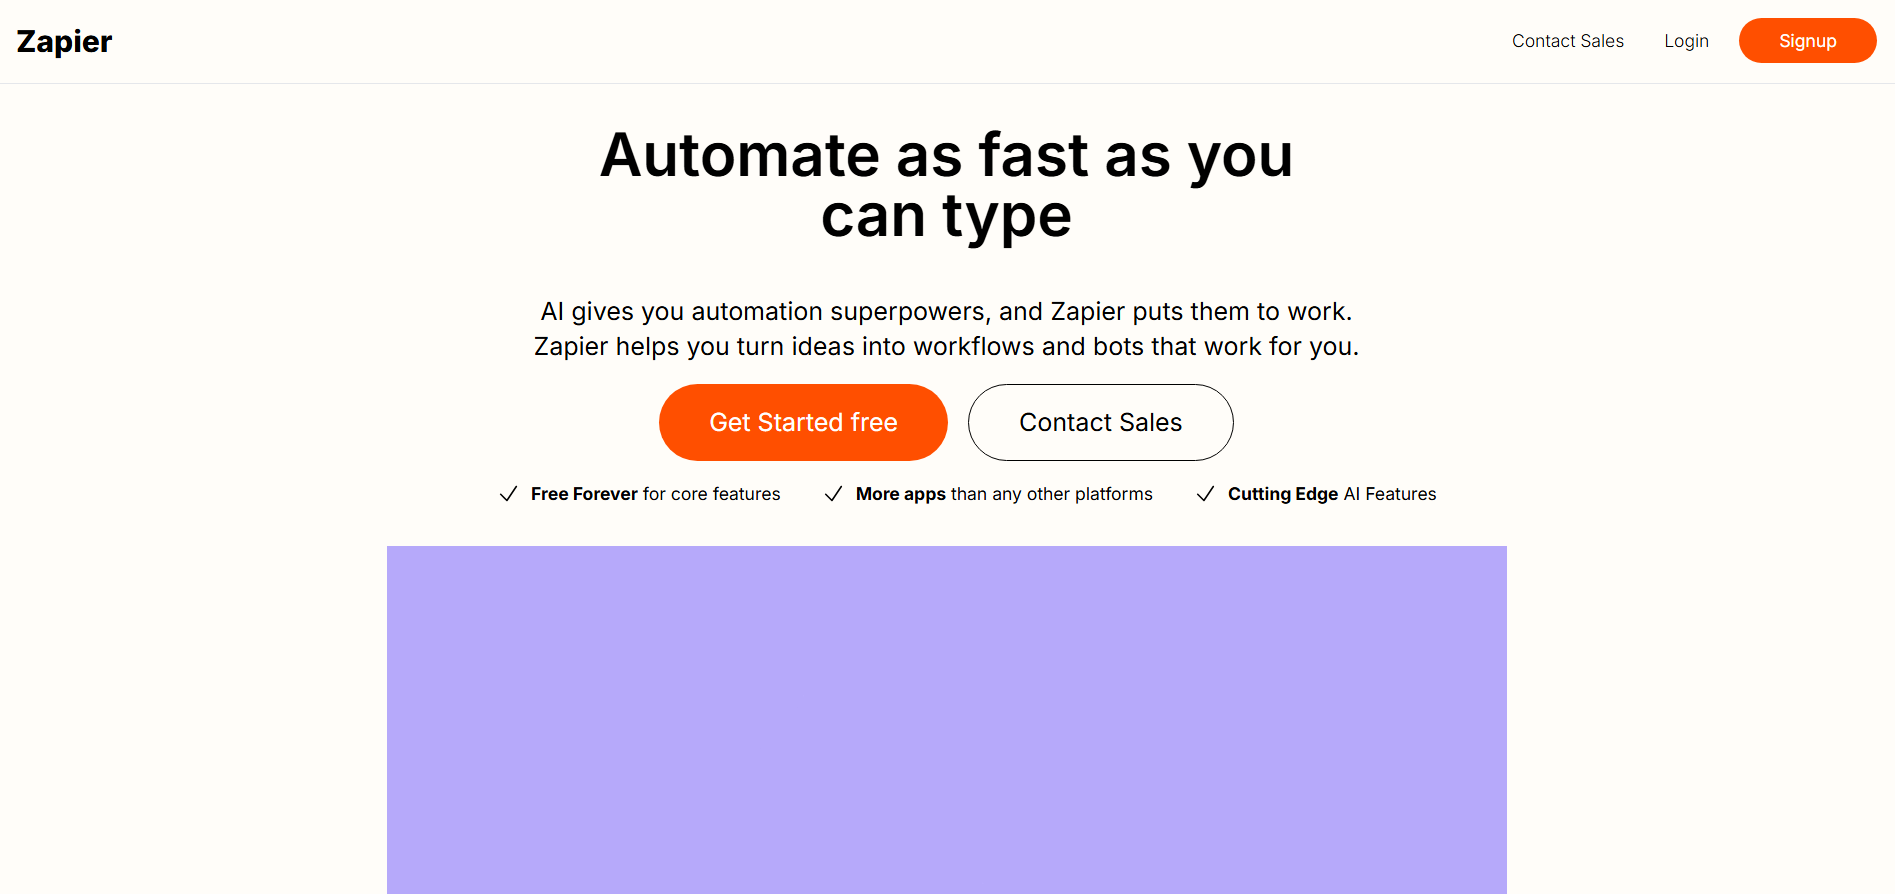
\includegraphics[width=\linewidth]{figures/ui-landing.png}\\[2pt]
    {\small\textbf{(a)} Landing page}
\end{minipage}\hfill
\begin{minipage}[t]{0.48\textwidth}
    \centering
    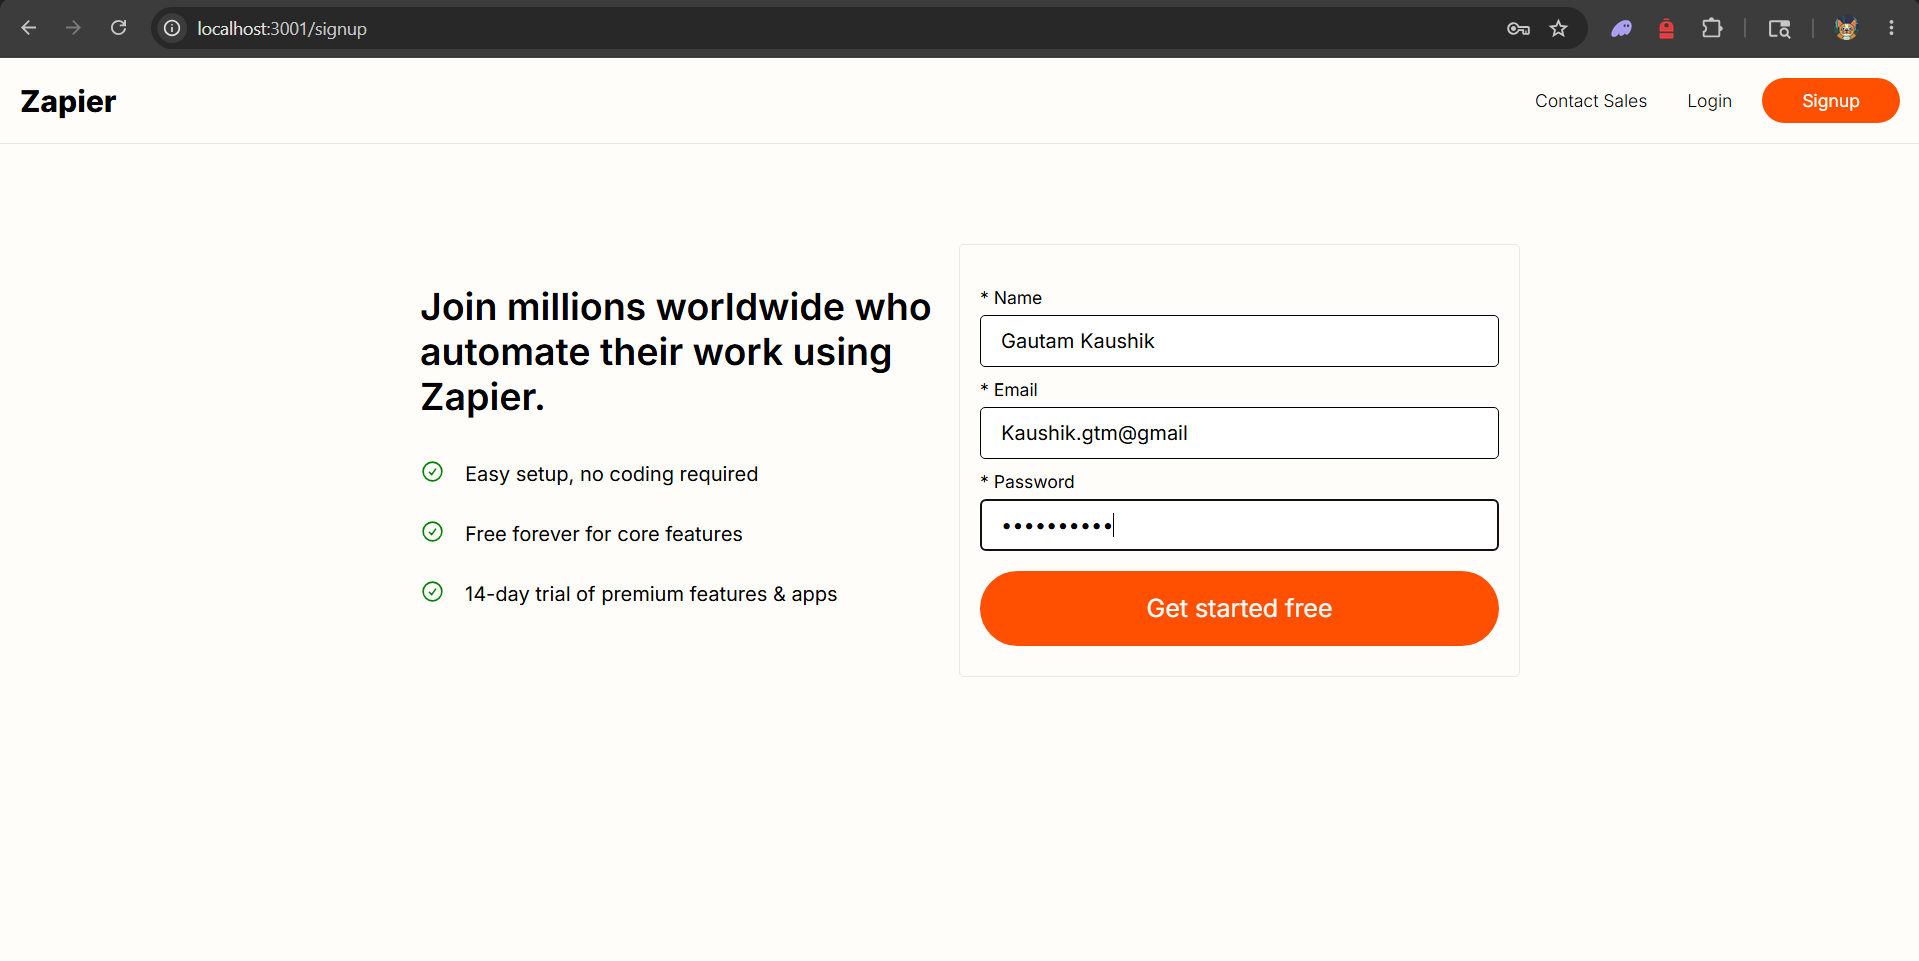
\includegraphics[width=\linewidth]{figures/ui-signup.png}\\[2pt]
    {\small\textbf{(b)} Signup form}
\end{minipage}
\caption{Public-facing frontend pages. The landing page (a) is the unauthenticated entry point; the signup form (b) posts to \texttt{POST /api/v1/user/signup}, after which the user is redirected to the dashboard.}
\label{fig:ui-public}
\end{figure}

\begin{figure}[h]
\centering
\begin{minipage}[t]{0.48\textwidth}
    \centering
    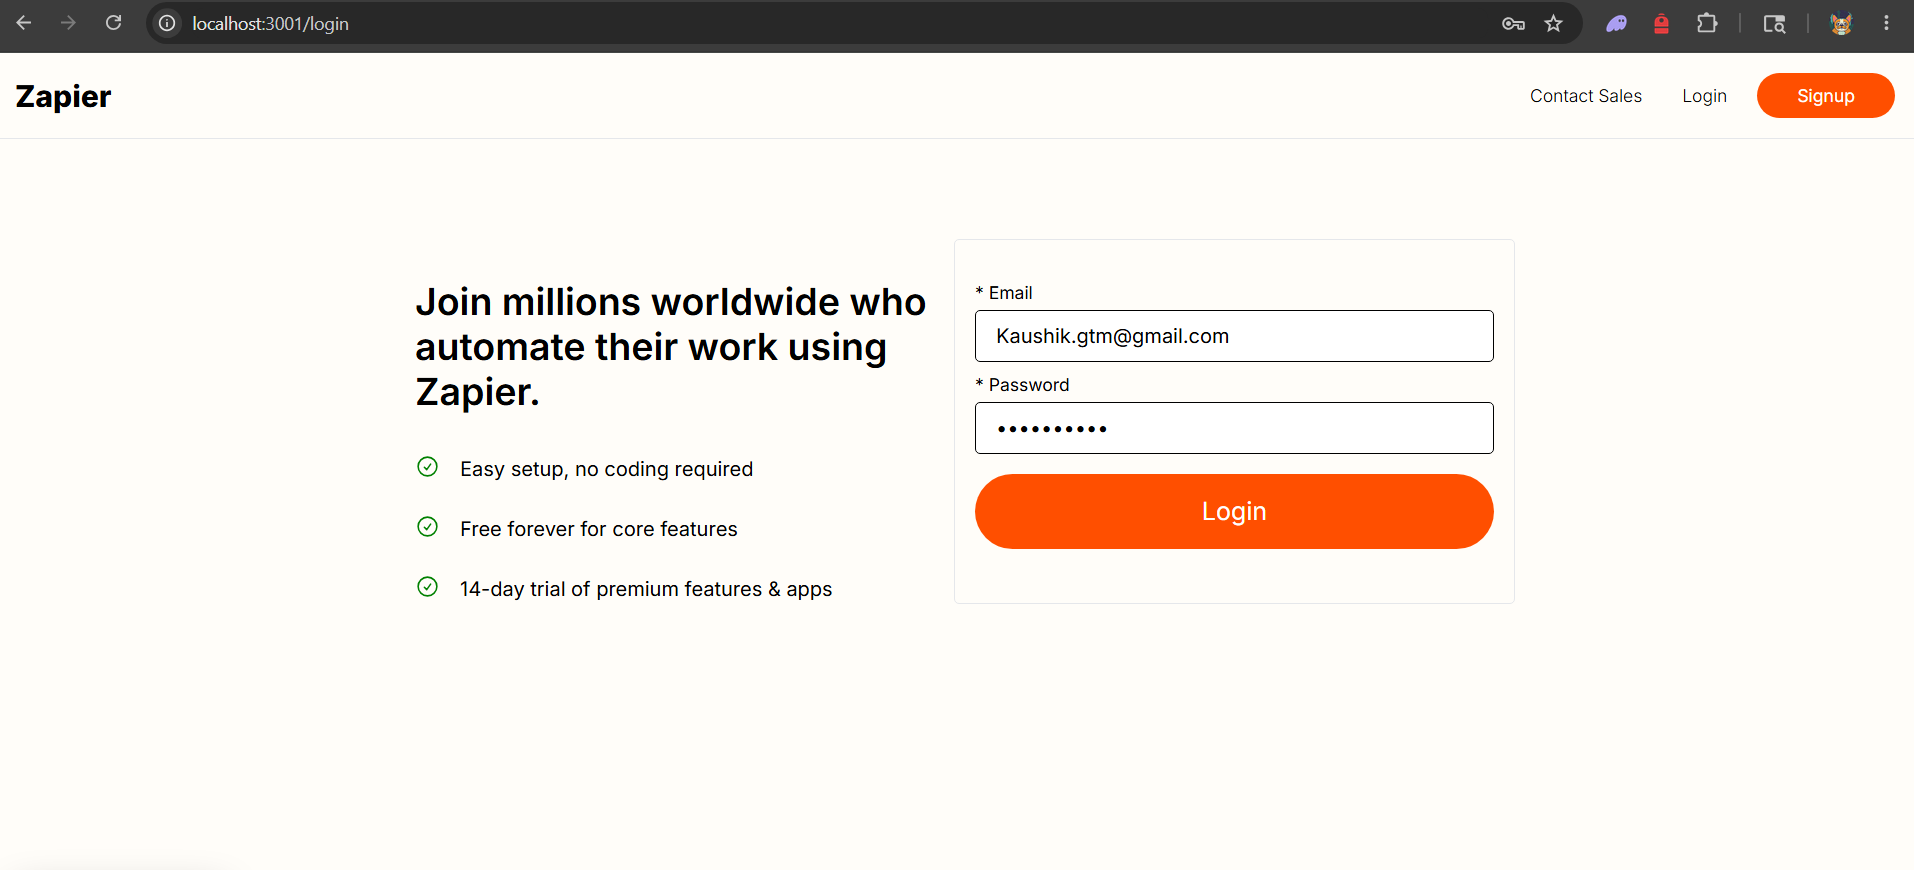
\includegraphics[width=\linewidth]{figures/ui-login.png}\\[2pt]
    {\small\textbf{(a)} Sign-in form}
\end{minipage}\hfill
\begin{minipage}[t]{0.48\textwidth}
    \centering
    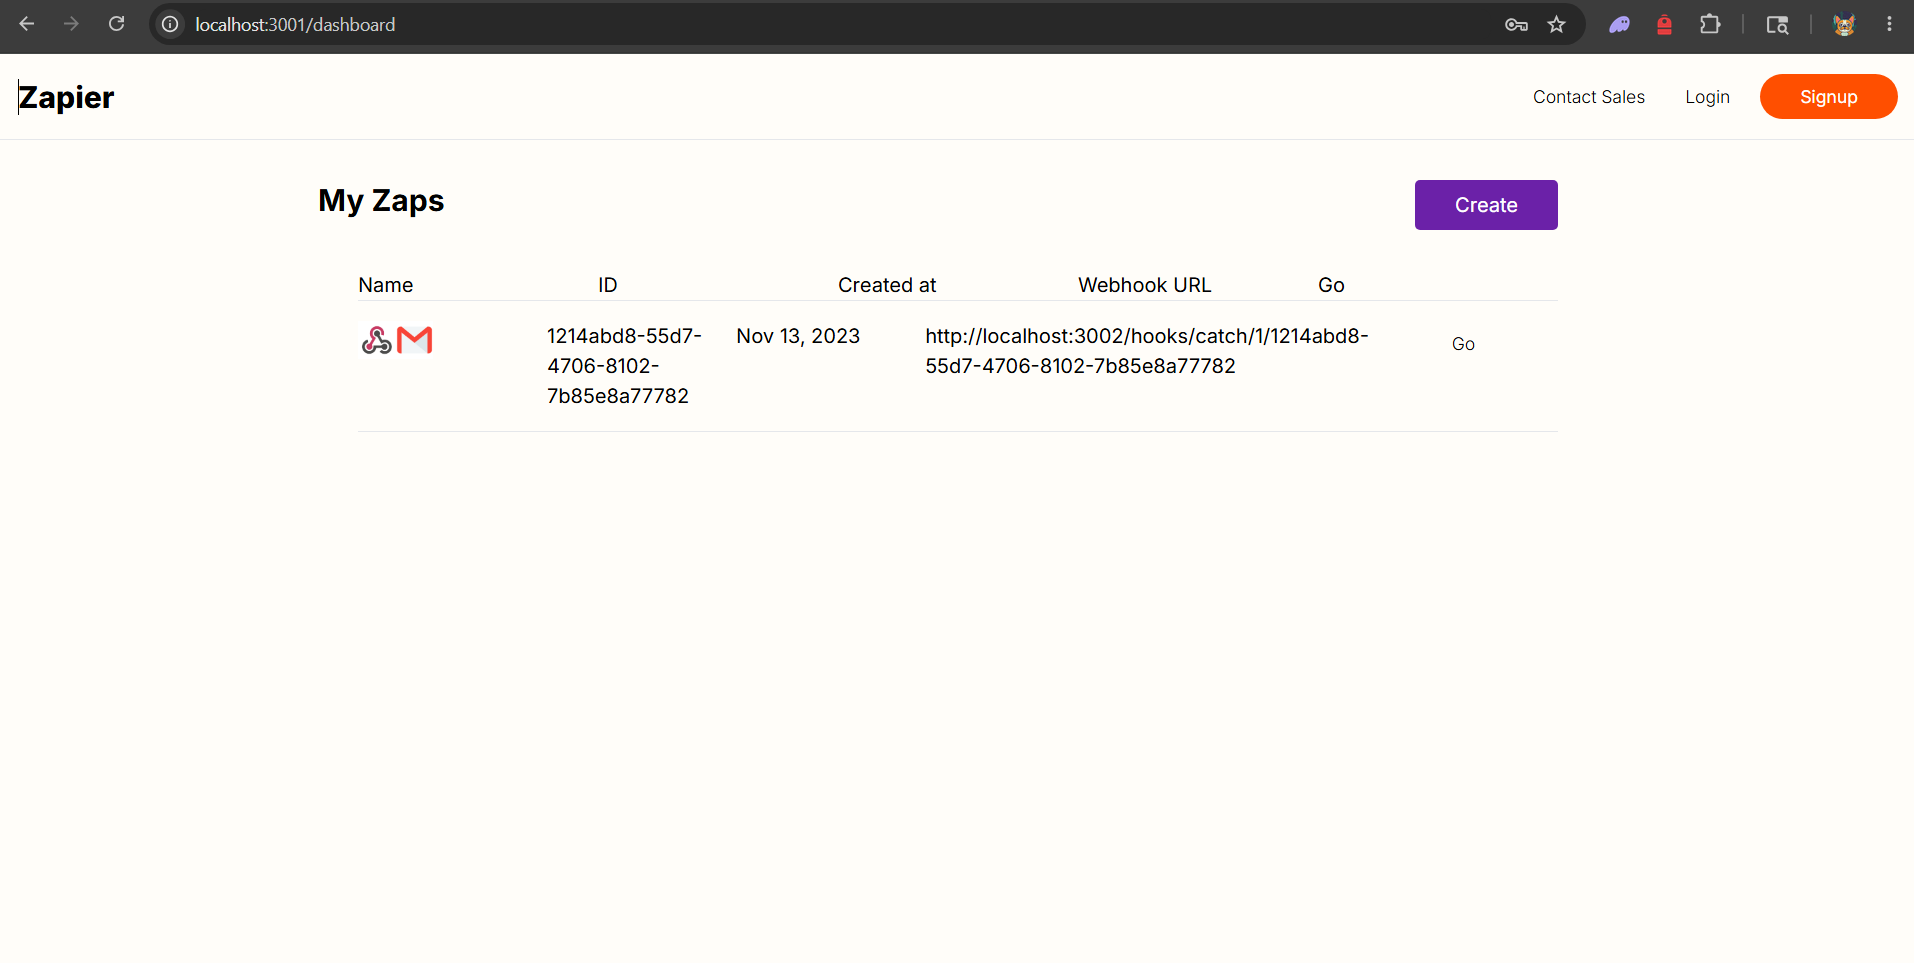
\includegraphics[width=\linewidth]{figures/ui-dashboard.png}\\[2pt]
    {\small\textbf{(b)} Dashboard listing the user's Zaps}
\end{minipage}
\caption{Authenticated user surfaces. Submitting the sign-in form (a) issues a JWT that is attached to all subsequent API calls; the dashboard (b) lists each Zap together with its unique public webhook URL that external systems can POST to in order to fire the workflow.}
\label{fig:ui-auth}
\end{figure}

\begin{figure}[h]
\centering
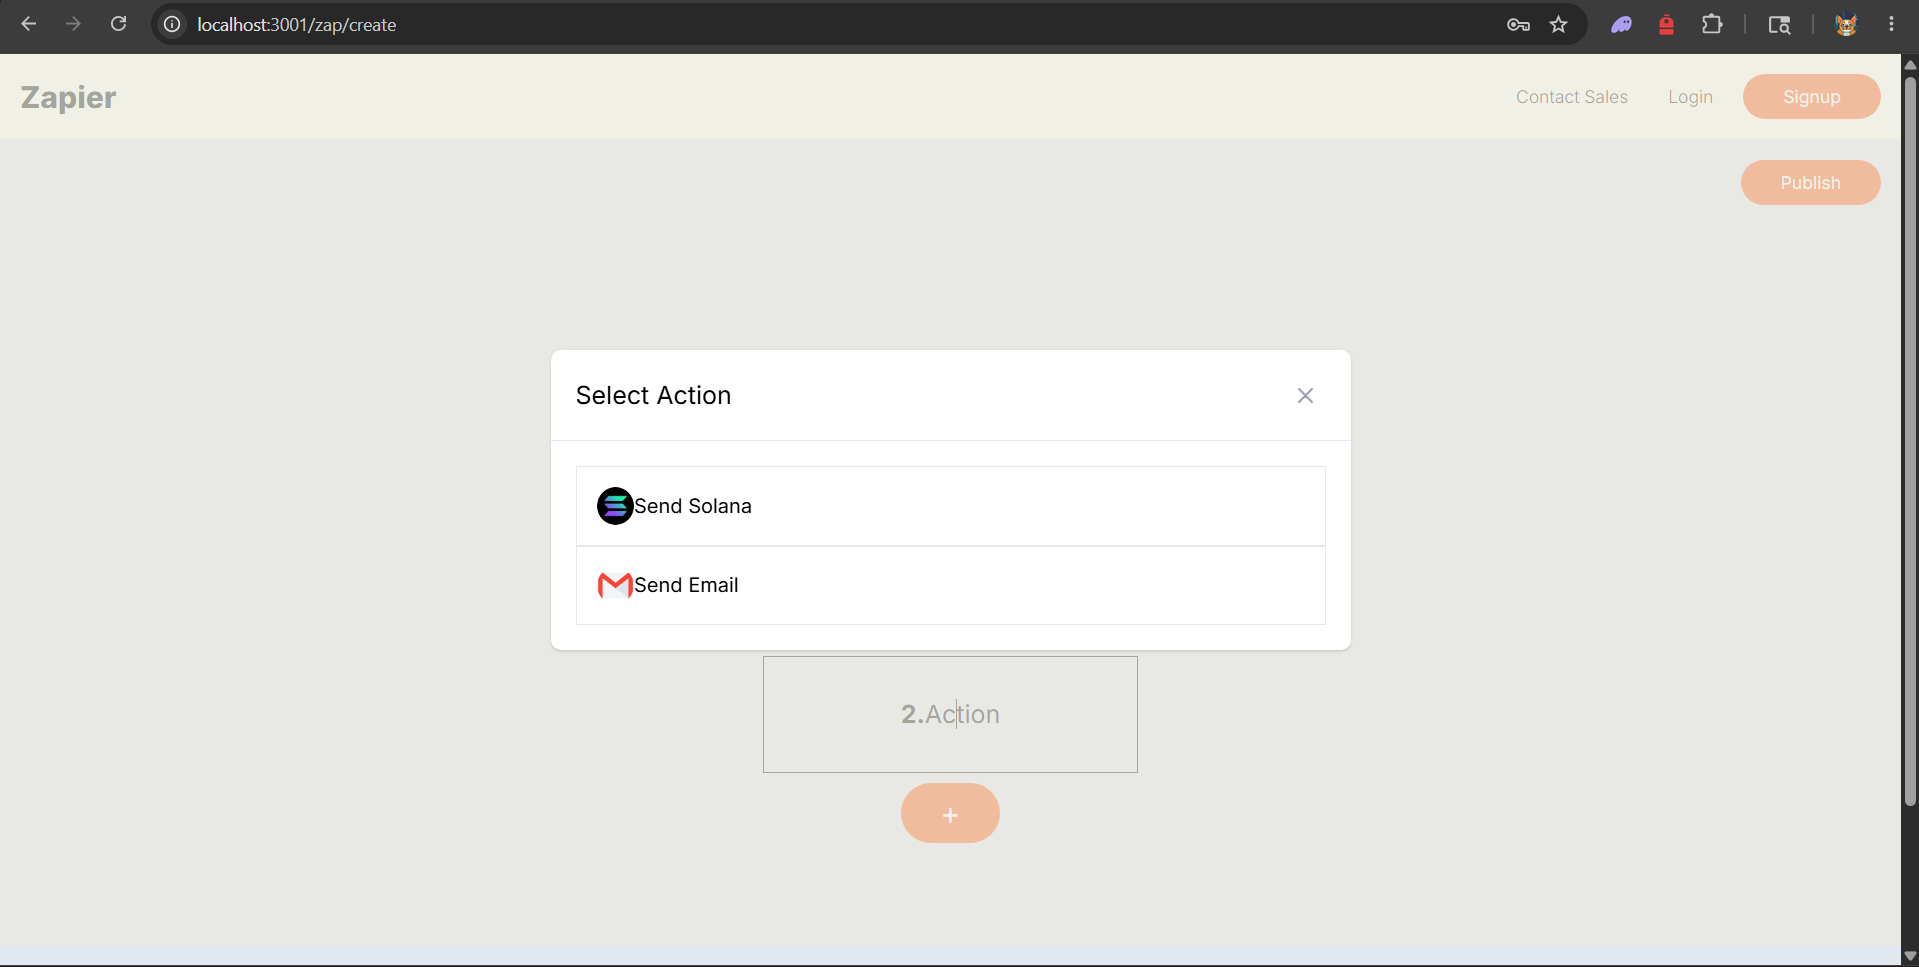
\includegraphics[width=0.9\textwidth]{figures/ui-zap-builder.png}
\caption{The Zap-builder screen with the action-selection modal open. Available actions are fetched dynamically from \texttt{GET /api/v1/action/available}, so adding a new server-side action type makes it immediately selectable in the UI without any frontend change.}
\label{fig:ui-zap-builder}
\end{figure}

Every service is containerised using a dedicated \texttt{Dockerfile} and can be brought up locally using the provided \texttt{docker-compose.yml}, which additionally launches a single-broker Kafka cluster (with Zookeeper) on port 9092. A second compose file, \texttt{docker-compose.prod.yml}, references pre-built images from Docker Hub and is intended for production deployment on a single virtual machine. Figure~\ref{fig:cicd} shows the structure of the CI/CD pipeline, which is implemented as a GitHub Actions workflow. On each push to \texttt{main}, the pipeline first detects which service directories have changed, then builds and pushes a new Docker image to Docker Hub for each changed service, and finally connects to the deployment host over SSH and restarts only the containers whose images were rebuilt. This strategy keeps deployments fast and minimises downtime.

\begin{figure}[h]
\centering
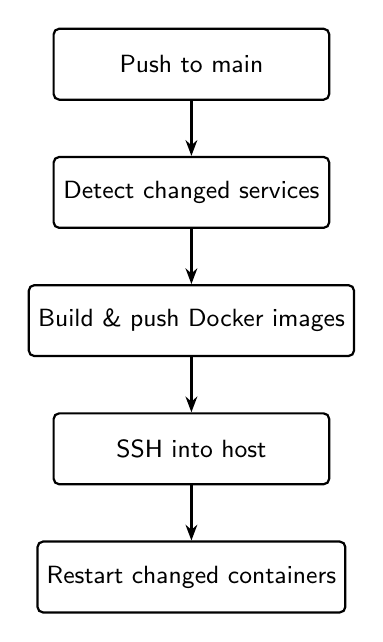
\begin{tikzpicture}[
    node distance=0.7cm,
    box/.style={draw, thick, minimum width=3.5cm, minimum height=0.9cm, align=center, rounded corners=2pt, font=\small},
    >={Stealth[length=2mm]}
]
\node[box] (push) {Push to main};
\node[box, below=of push] (detect) {Detect changed services};
\node[box, below=of detect] (build) {Build \& push Docker images};
\node[box, below=of build] (deploy) {SSH into host};
\node[box, below=of deploy] (restart) {Restart changed containers};

\draw[->, thick] (push) -- (detect);
\draw[->, thick] (detect) -- (build);
\draw[->, thick] (build) -- (deploy);
\draw[->, thick] (deploy) -- (restart);
\end{tikzpicture}
\caption{Continuous integration and deployment pipeline.}
\label{fig:cicd}
\end{figure}
     % Chapter 4
\chapter{Discussion of Results}

\section{Verification Methodology}

The platform was deployed locally using Docker Compose on a developer workstation, with all five services and the Kafka and PostgreSQL containers running on the same host. Each functional capability described in Chapter~4 was exercised through the web frontend, and the corresponding internal state, including database rows, Kafka topic offsets and service log lines, was inspected to verify correctness. In addition to the positive functional tests, two simulated failure scenarios were carried out: the processor service was stopped while webhooks continued to arrive, and the worker service was crashed mid-execution in order to confirm that no events were lost and that re-delivery semantics held.

\section{Functional Results}

The functional outcomes of these tests are summarised in Table~\ref{tab:results}. All ten of the scenarios that were executed produced the expected outcome, confirming that the platform meets the functional and non-functional requirements set out in Chapter~3.

\begin{table}[h]
\centering
\caption{Functional verification results.}
\label{tab:results}
\renewcommand{\arraystretch}{1.3}
\begin{tabular}{|p{6.0cm}|p{2.0cm}|p{5.0cm}|}
\hline
\textbf{Test scenario} & \textbf{Outcome} & \textbf{Observation} \\ \hline
User signup with valid input & Pass & New \texttt{User} row created, password stored as a bcrypt hash. \\ \hline
User signin with valid credentials & Pass & JWT issued; subsequent authenticated requests accepted. \\ \hline
User signin with invalid credentials & Pass & Request rejected with HTTP 403. \\ \hline
Creation of a Zap with one trigger and two actions & Pass & \texttt{Zap}, \texttt{Trigger} and two \texttt{Action} rows persisted in a single transaction. \\ \hline
Webhook invocation on the public URL & Pass & \texttt{ZapRun} and \texttt{ZapRunOutbox} rows inserted atomically. \\ \hline
Processor pickup of a new outbox row & Pass & Row read, message published to Kafka, row deleted within the next polling interval. \\ \hline
Worker execution of an email action & Pass & Email delivered to the recipient with placeholders correctly substituted. \\ \hline
Worker execution of a chained second action & Pass & Follow-up Kafka message produced and consumed; second action executed in order. \\ \hline
Webhook arrival while processor is offline & Pass & Outbox rows accumulated; on restart, the rows were processed and no events were lost. \\ \hline
Worker crash mid-execution & Pass & On restart, the un-acknowledged Kafka message was re-delivered and the action was re-executed. \\ \hline
\end{tabular}
\end{table}

Figure~\ref{fig:result-email} shows direct end-to-end evidence of the platform's correctness: a transactional email produced by the worker's \texttt{email} action and delivered to the recipient's mailbox after the corresponding Zap was fired by a webhook.

\begin{figure}[h]
\centering
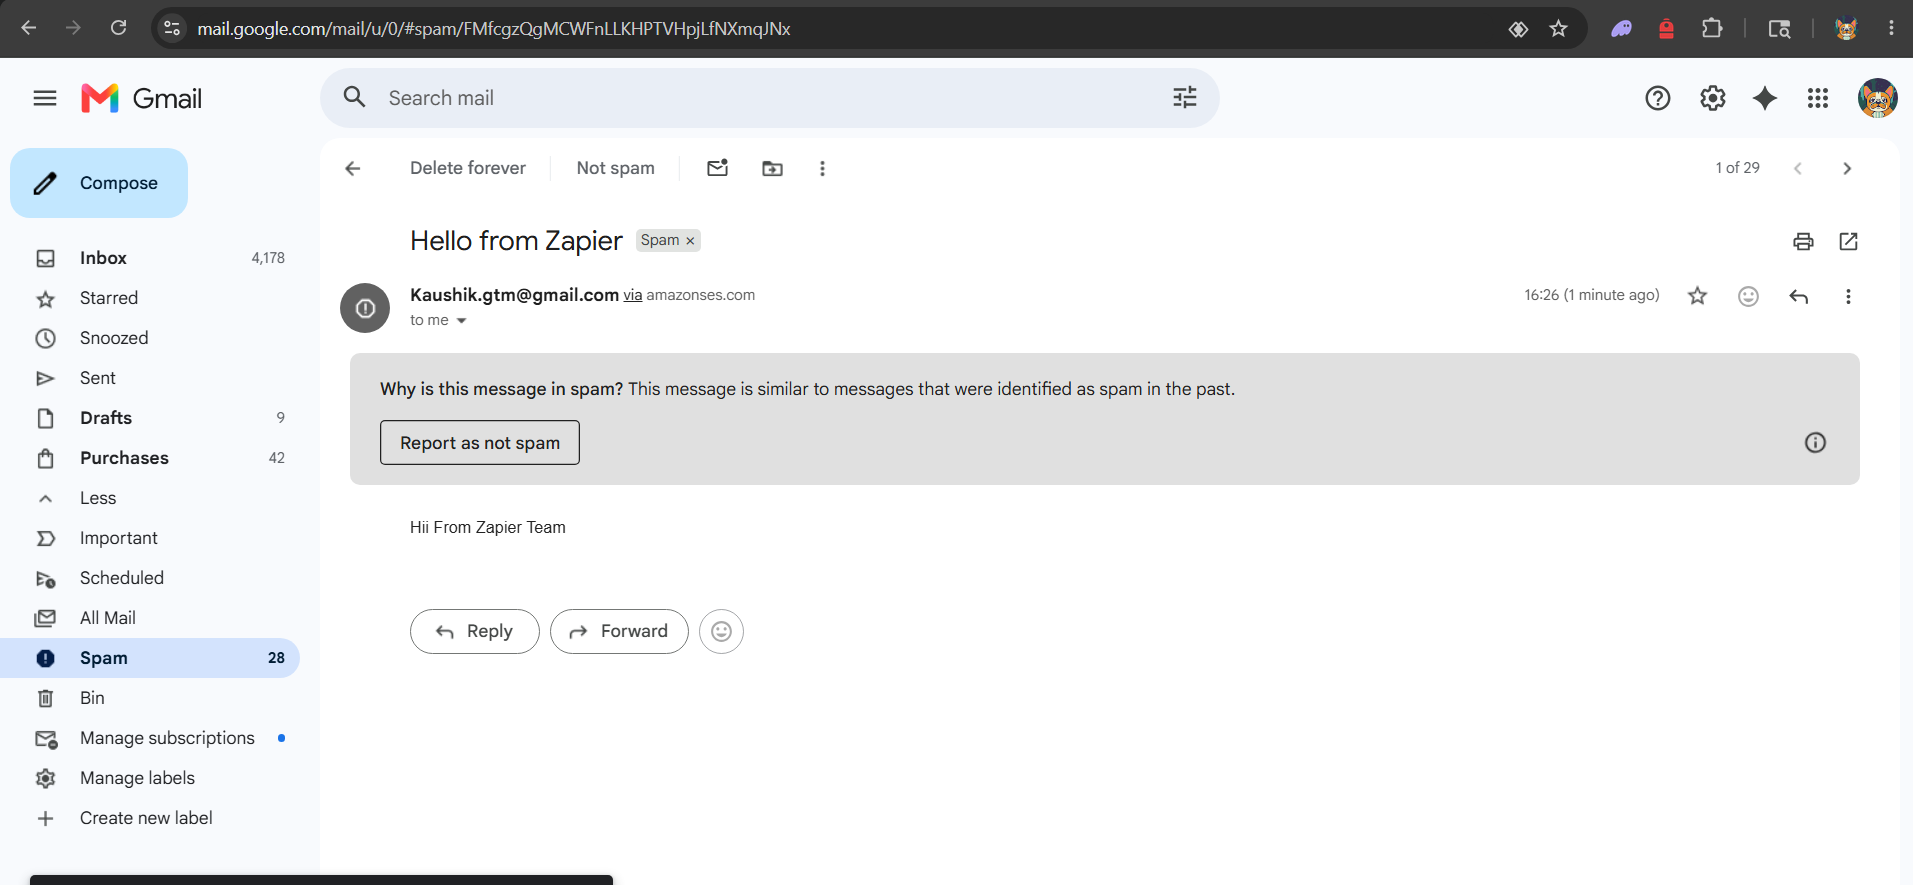
\includegraphics[width=0.95\textwidth]{figures/result-email-delivered.png}
\caption{End-to-end verification of the \texttt{email} action: a message produced by the worker, relayed over SMTP through the configured transactional-email provider, and received in the recipient's Gmail inbox. The full path exercised here is hook $\rightarrow$ outbox $\rightarrow$ processor $\rightarrow$ Kafka $\rightarrow$ worker $\rightarrow$ SMTP. The ``Why is this message in spam?'' banner is Gmail's automated heuristic for unverified senders and does not affect delivery.}
\label{fig:result-email}
\end{figure}

\section{Qualitative Observations}

\subsection{Latency}

End-to-end latency from webhook reception to first-action execution, measured informally with timestamped log lines on the development workstation, was consistently below two seconds. The dominant contributor to this latency was the processor's polling interval, which had been deliberately set to two seconds in order to keep the processor's load on the database low. Reducing this interval would lower the observed latency proportionally, at the cost of additional database queries even when the outbox table is empty.

\subsection{Throughput}

The throughput of the system was not stress-tested at scale, but the architecture imposes no inherent bottleneck other than the database itself. The worker can be scaled horizontally by adding more consumer-group members; Kafka automatically rebalances partitions across the new instances. The processor can be partitioned in the same way by sharding the outbox table or by running multiple processor instances configured to handle different ranges of the outbox primary key. Both the API and the hook services are stateless and can be replicated behind a load balancer.

\subsection{Reliability}

The two simulated failure scenarios in Table~\ref{tab:results} are the most important qualitative outcomes. They demonstrate that the transactional outbox pattern, together with manual Kafka offset commits in the worker, gives the platform the at-least-once delivery semantics specified in the non-functional requirements. In no test did a webhook event acknowledged with HTTP 200 fail to result in the eventual execution of its associated actions.

\subsection{Developer Experience}

A secondary but important outcome was the developer experience of the system. The whole platform comes up with a single \texttt{docker compose up} command, and the modular separation between services means that an engineer working on, for example, the worker can restart only that one container without affecting the rest. The use of TypeScript across the entire codebase eliminated an entire class of bugs related to property-name typos and mismatched payload shapes during integration testing.

\section{Comparison with Stated Requirements}

Table~\ref{tab:req-compliance} maps each requirement from Chapter~3 to the corresponding test scenario or implementation evidence that satisfies it. Every requirement listed is fully satisfied by the present implementation.

\begin{table}[h]
\centering
\caption{Mapping of requirements to verification evidence.}
\label{tab:req-compliance}
\renewcommand{\arraystretch}{1.3}
\begin{tabular}{|p{2.0cm}|p{6.0cm}|p{5.5cm}|}
\hline
\textbf{Req.\ ID} & \textbf{Requirement (abridged)} & \textbf{Evidence} \\ \hline
FR-1 & User signup and authentication & Tests rows 1--3, Table~\ref{tab:results} \\ \hline
FR-3 & CRUD on Zaps & Test row 4, Table~\ref{tab:results} \\ \hline
FR-4 & Unique webhook URL per Zap & Hook route \texttt{/hooks/catch/:userId/:zapId} \\ \hline
FR-5 & Actions execute in order & Test row 8, Table~\ref{tab:results} \\ \hline
FR-6 & Email and Solana actions & Worker action types, Ch.\ 4, Table 4.3 \\ \hline
FR-7 & Template substitution & Email test row 7, Table~\ref{tab:results} \\ \hline
NFR-1 & Durability across broker outages & Test row 9, Table~\ref{tab:results} \\ \hline
NFR-2 & At-least-once execution & Test row 10, Table~\ref{tab:results} \\ \hline
NFR-3 & Ordered execution & Test row 8, Table~\ref{tab:results} \\ \hline
NFR-4 & Horizontal scalability & Kafka consumer group, Ch.\ 4, \S Worker \\ \hline
NFR-6 & Single-command local startup & \texttt{docker compose up} \\ \hline
NFR-7 & Password hashing and JWT auth & Test rows 1--3, Table~\ref{tab:results} \\ \hline
\end{tabular}
\end{table}
 % Chapter 5
\chapter{Conclusion and Future Work}

\section{Conclusion}

This project has presented the design, implementation and verification of an open, self-hostable workflow automation platform built as a small set of cooperating microservices. The platform satisfies the functional objectives stated in Chapter~1 and the explicit functional and non-functional requirements set out in Chapter~3: users can register and authenticate, define workflows consisting of a webhook trigger and an ordered chain of actions, invoke those workflows from external systems, and observe the actions being executed reliably and in order.

The most significant architectural decision in the project was the adoption of the transactional outbox pattern for the webhook ingestion path. By inserting both the business state change and the outbox entry in a single database transaction, the platform side-steps the dual-write problem that otherwise plagues integrations between a relational database and a message broker, and obtains \emph{at-least-once} delivery semantics for every event without requiring a distributed transaction coordinator. The complementary use of Apache Kafka as the asynchronous channel between the processor and the worker, together with manual offset commits in the worker, propagates the same delivery guarantee through the entire execution pipeline.

The implementation also demonstrates that a modern microservices architecture can be built with a relatively small codebase. Each individual service is small enough to be read and understood in a single sitting; the complexity of the system as a whole arises from the interactions between services rather than from any one of them. The TypeScript-on-Node.js stack, combined with Prisma's typed query builder, kept integration friction low and made it possible for a small team to evolve the schema, the API, the workers and the frontend in parallel without breaking each other's work.

Beyond the artefact itself, the project has given the team direct exposure to the design and operation of distributed systems. The team has practised relational schema design, asynchronous programming, container orchestration, continuous deployment with GitHub Actions, and the operational reality of a system in which failures occur and must be tolerated rather than prevented. These are the same skills required of a contemporary professional software engineer.

\section{Limitations of the Current Implementation}

A number of limitations of the present implementation should be acknowledged. First, the platform supports only a single trigger type (incoming webhook) and only two action types (email and Solana transfer); a commercially competitive platform would need to support several hundred integrations. Second, the processor's polling loop, although adequate for the present scale, introduces an avoidable latency of up to two seconds per event; a change-data-capture stream would eliminate this. Third, the worker treats every failure as transient and relies on Kafka re-delivery for retry; there is no dead-letter queue or exponential back-off, which means that a permanently failing action will be retried indefinitely. Fourth, the deployment topology assumes a single virtual machine: there is no orchestration of multiple worker instances, no autoscaling and no production-grade secrets management.

\section{Future Work}

Several concrete enhancements have been identified for future iterations of the platform:

\begin{enumerate}[label=(\alph*)]
\item \textbf{Action catalogue.} Add additional action types that integrate with widely used SaaS systems such as Slack, Discord, Google Sheets, HubSpot and GitHub. Each new action requires only an action handler in the worker plus a row in the \texttt{AvailableAction} table.
\item \textbf{Scheduled and polling triggers.} Add trigger types that fire on a cron schedule or that periodically poll an external API for changes, in addition to the present webhook trigger.
\item \textbf{Change-data-capture for the outbox.} Replace the processor's polling loop with a Debezium connector that streams new outbox rows out of the PostgreSQL write-ahead log directly to Kafka, reducing the per-event latency to milliseconds.
\item \textbf{Dead-letter queue and retry policy.} Add a dedicated Kafka topic that receives messages whose execution has failed a configurable number of times, and expose a UI for human operators to inspect and replay them.
\item \textbf{Observability.} Instrument every service with OpenTelemetry traces and Prometheus metrics, and provide a Grafana dashboard that visualises end-to-end execution latency and per-action error rates.
\item \textbf{Security hardening.} Add rate limiting on the webhook endpoint, signature verification for incoming webhooks, secrets management through HashiCorp Vault, and TLS termination in front of all public-facing services.
\item \textbf{Kubernetes deployment.} Replace the Docker Compose deployment with a set of Kubernetes manifests, allowing multi-node deployment, autoscaling of the worker based on Kafka consumer lag, and rolling upgrades with zero downtime.
\item \textbf{Run history and analytics.} Extend the frontend with a dedicated view that lists each \texttt{ZapRun}, the actions that were executed for it, and the timestamp and outcome of each. This requires no schema change because every \texttt{ZapRun} is already persisted.
\end{enumerate}

Taken together, these enhancements would move the platform from a working reference implementation to a production-ready workflow automation product. Even without them, the platform as it stands serves both as a usable automation tool in its own right and as a compact, end-to-end reference implementation of an event-driven microservices architecture suitable for use in undergraduate and postgraduate courses on distributed systems.
            % Chapter 6

%==========================================================
%  REFERENCES (IEEE style)
%==========================================================
% Rename the auto-generated chapter heading of thebibliography from
% "Bibliography" (default) to "References".
\renewcommand{\bibname}{References}

% IEEE reference style: numeric citations, numbered list.
% Each entry is followed by a one-line annotation in italic indicating the
% type of source (book / journal / RFC / online documentation / industry article)
% and where in this project it was consulted.

{\setstretch{1.0}
\small
\begin{thebibliography}{99}
\addcontentsline{toc}{chapter}{References}
\markboth{REFERENCES}{REFERENCES}
\setlength{\itemsep}{2pt}

\bibitem{fowler2014microservices}
M.~Fowler and J.~Lewis, ``Microservices: A definition of this new architectural term,'' \emph{martinfowler.com}, Mar. 2014. [Online]. Available: \url{https://martinfowler.com/articles/microservices.html}.\\
\textit{Industry article; foundational definition of the microservices style, consulted while designing the five-service decomposition in Ch.~4.}

\bibitem{richardson2018microservices}
C.~Richardson, \emph{Microservices Patterns: With Examples in Java}. Shelter Island, NY, USA: Manning Publications, 2018, ch.~3, ``Transactional Outbox Pattern''.\\
\textit{Reference textbook; primary source for the transactional outbox pattern applied in the hook service (Ch.~2 \S 3, Ch.~4 \S Hook).}

\bibitem{microservicesio_outbox}
C.~Richardson, ``Pattern: Transactional outbox,'' \emph{microservices.io}, 2017. [Online]. Available: \url{https://microservices.io/patterns/data/transactional-outbox.html}.\\
\textit{Online pattern catalogue; complements~\cite{richardson2018microservices} with a concise specification of the outbox-poller variant we implemented.}

\bibitem{kleppmann2017dia}
M.~Kleppmann, \emph{Designing Data-Intensive Applications}. Sebastopol, CA, USA: O'Reilly Media, 2017.\\
\textit{Reference textbook; consulted for the discussion of dual-write inconsistency, at-least-once delivery and stream-processing trade-offs (Ch.~2--3).}

\bibitem{narkhede2017kafka}
N.~Narkhede, G.~Shapira, and T.~Palino, \emph{Kafka: The Definitive Guide}. Sebastopol, CA, USA: O'Reilly Media, 2017.\\
\textit{Reference textbook; consumer-group rebalancing and manual-offset semantics described here directly informed the worker design (Ch.~4 \S Worker).}

\bibitem{kafka_docs}
Apache Software Foundation, ``Apache Kafka documentation,'' 2024. [Online]. Available: \url{https://kafka.apache.org/documentation/}.\\
\textit{Official documentation; authoritative source for Kafka producer/consumer APIs and broker configuration used in the processor and worker services.}

\bibitem{kreps2014log}
J.~Kreps, ``The log: What every software engineer should know about real-time data's unifying abstraction,'' \emph{LinkedIn Engineering Blog}, Dec. 2013. [Online]. Available: \url{https://engineering.linkedin.com/distributed-systems/log-what-every-software-engineer-should-know-about-real-time-datas-unifying}.\\
\textit{Industry article; conceptual framing of the partitioned-log abstraction that motivates the use of Kafka in Ch.~2.}

\bibitem{jones2015jwt}
M.~Jones, J.~Bradley, and N.~Sakimura, \emph{JSON Web Token (JWT)}, RFC~7519, Internet Engineering Task Force, May 2015. [Online]. Available: \url{https://www.rfc-editor.org/rfc/rfc7519}.\\
\textit{IETF standard (RFC); normative specification for the JWT format issued by the primary backend after successful sign-in (Ch.~4 \S Primary Backend).}

\bibitem{provos1999bcrypt}
N.~Provos and D.~Mazi\`{e}res, ``A future-adaptable password scheme,'' in \emph{Proc.\ USENIX Annual Technical Conference, FREENIX Track}, Monterey, CA, USA, Jun. 1999, pp.~81--91.\\
\textit{Peer-reviewed conference paper; original description of the bcrypt password-hashing algorithm used to store user passwords (NFR-7).}

\bibitem{fielding2000rest}
R.~T.~Fielding, ``Architectural styles and the design of network-based software architectures,'' Ph.D.\ dissertation, Univ.\ of California, Irvine, CA, USA, 2000.\\
\textit{Doctoral dissertation; canonical formulation of the REST style that shapes the primary backend's HTTP endpoint design (Ch.~4 Table~4.2).}

\bibitem{postgresql_docs}
PostgreSQL Global Development Group, ``PostgreSQL 16 documentation,'' 2024. [Online]. Available: \url{https://www.postgresql.org/docs/16/}.\\
\textit{Official documentation; consulted for transaction isolation guarantees relied on by the hook's \texttt{\$transaction} block (Ch.~4 \S Hook).}

\bibitem{prisma_docs}
Prisma Data, Inc., ``Prisma ORM documentation,'' 2024. [Online]. Available: \url{https://www.prisma.io/docs}.\\
\textit{Official documentation; primary reference for schema modelling, migrations and the typed query API used across all backend services.}

\bibitem{nextjs_docs}
Vercel, Inc., ``Next.js documentation,'' 2024. [Online]. Available: \url{https://nextjs.org/docs}.\\
\textit{Official documentation; used for App-Router conventions, server components and styling integration in the frontend (Ch.~4 \S Frontend).}

\bibitem{express_docs}
OpenJS Foundation, ``Express -- Node.js web application framework,'' 2024. [Online]. Available: \url{https://expressjs.com/}.\\
\textit{Official documentation; reference for routing, middleware composition and request validation in the primary backend and hook services.}

\bibitem{nodemailer_docs}
A.~Reinman, ``Nodemailer -- Send e-mails with Node.js,'' 2024. [Online]. Available: \url{https://nodemailer.com/}.\\
\textit{Library documentation; reference for SMTP transport configuration used by the worker's \texttt{email} action.}

\bibitem{solana_web3}
Solana Labs, ``@solana/web3.js library documentation,'' 2024. [Online]. Available: \url{https://solana-labs.github.io/solana-web3.js/}.\\
\textit{Library documentation; reference for transaction construction and signing used by the worker's \texttt{send-sol} action.}

\bibitem{docker_docs}
Docker, Inc., ``Docker and Docker Compose documentation,'' 2024. [Online]. Available: \url{https://docs.docker.com/}.\\
\textit{Official documentation; basis for the per-service \texttt{Dockerfile}s and the \texttt{docker-compose.yml} orchestration described in Ch.~4 \S Frontend and Deployment.}

\bibitem{typescript_docs}
Microsoft Corporation, ``TypeScript handbook,'' 2024. [Online]. Available: \url{https://www.typescriptlang.org/docs/}.\\
\textit{Official documentation; language reference for the TypeScript codebase shared across all five services.}

\bibitem{zod_docs}
C.~McDonnell, ``Zod -- TypeScript-first schema validation,'' 2024. [Online]. Available: \url{https://zod.dev/}.\\
\textit{Library documentation; reference for input-schema validation used by every authenticated endpoint of the primary backend.}

\bibitem{github_actions_docs}
GitHub, Inc., ``GitHub Actions documentation,'' 2024. [Online]. Available: \url{https://docs.github.com/en/actions}.\\
\textit{Official documentation; basis for the change-detection and deploy workflow shown in Figure~4.4 (CI/CD pipeline).}

\end{thebibliography}
}% end \setstretch group


%==========================================================
%  APPENDICES
%==========================================================
\appendix
\chapter{Environment Variables}

The following environment variables are required by the platform's services. They are typically supplied through a \texttt{.env} file in each service directory, and Docker Compose forwards them into the corresponding container at startup. The variables are summarised in Table~\ref{tab:env}.

\begin{table}[h]
\centering
\caption{Environment variables used by the platform.}
\label{tab:env}
\renewcommand{\arraystretch}{1.3}
\begin{tabular}{|p{3.8cm}|p{4.5cm}|p{5cm}|}
\hline
\textbf{Variable} & \textbf{Used by} & \textbf{Purpose} \\ \hline
\texttt{DATABASE\_URL} & primary backend, hook, worker & PostgreSQL connection string. \\ \hline
\texttt{JWT\_PASSWORD} & primary backend & Secret used to sign and verify JSON Web Tokens. \\ \hline
\texttt{KAFKA\_BROKERS} & processor, worker & Comma-separated list of Kafka broker addresses. \\ \hline
\texttt{SMTP\_ENDPOINT} & worker & Hostname of the SMTP relay used for email actions. \\ \hline
\texttt{SMTP\_USERNAME} & worker & Username for the SMTP relay. \\ \hline
\texttt{SMTP\_PASSWORD} & worker & Password for the SMTP relay. \\ \hline
\texttt{SOL\_PRIVATE\_KEY} & worker & Base58-encoded private key of the funding Solana wallet. \\ \hline
\end{tabular}
\end{table}

\chapter{Sample Webhook Payload and Trace}
{\setstretch{1.25}

Listing~\ref{lst:sample-payload} shows a representative JSON payload that an external service might POST to a Zap's webhook URL. The corresponding sequence of state transitions observed inside the platform is shown immediately below.

\begin{lstlisting}[language=JavaScript, caption={Sample webhook payload.}, label=lst:sample-payload]
{
  "user":    { "email": "recipient@example.com", "name": "Asha" },
  "payment": { "amount": "0.25", "currency": "SOL" },
  "wallet":  { "address": "9xQeWvG816bUx9EPjHmaT23yvVM2Z7trM5HEzy" }
}
\end{lstlisting}

\begin{enumerate}[label=\arabic*., leftmargin=*, itemsep=2pt, parsep=2pt, topsep=2pt]
\item The hook service inserts one \texttt{ZapRun} row (with the payload above stored in the \texttt{metadata} column) and one \texttt{ZapRunOutbox} row, in a single Prisma transaction.
\item The processor, on its next poll, reads the outbox row and publishes the message \texttt{\{"zapRunId":"...","stage":0\}} to the \texttt{zap-events} Kafka topic, then deletes the outbox row.
\item The worker consumes the message, loads the \texttt{Zap} along with its actions, and executes the action at \texttt{sortingOrder} 0 (in this example, an email to \texttt{recipient@example.com}).
\item Because a second action exists, the worker publishes \texttt{\{"zapRunId":"...","stage":1\}} to Kafka and commits the offset of the first message.
\item The worker consumes the second message and executes the action at \texttt{sortingOrder} 1 (a Solana transfer of 0.25 SOL to the address contained in the payload). The offset is committed and processing of this \texttt{ZapRun} is complete.
\end{enumerate}
}% end \setstretch group


\end{document}
